\section{Explicación y descripción del tutorial}

La aplicación web que crearemos con la ayuda del tutorial de JDeveloper al que puede acceder si selecciona este \href{https://docs.oracle.com/cd/E53569_01/tutorials/tut_rich_app_alta/tut_rich_app_alta_1.html}{enlace}.

Para facilitar el trabajo hemos usado las mismas tablas de \texttt{stock}, \texttt{pedido} y \texttt{detalle\_pedido} del seminario 2.

\subsection{Crear una aplicación web fusion}
\begin{enumerate}
	\item Al iniciar JDeveloper seleccionaremos: Start $\rightarrow$ Programs $\rightarrow$ JDEVELOPER\_HOME $\rightarrow$ OracleHome $\rightarrow$ Oracle JDeveloper Studio $\rightarrow$ Oracle JDeveloper Studio
	\item Como no queremos ningún rol específico seleccionaremos Studio Developer (All Features) $\rightarrow$ OK.
	\item Nos sale un cuadro de diálogo preguntándonos si deseamos preferencias de importación de una instalación anterior $\rightarrow$ le damos a No.
	\item Nos sale otra ventana emergente sobre la política de privacidad $\rightarrow$ le damos a Aceptar.
	\item Nos aparece la página de inicio.
	\item Seleccionamos: Application $\rightarrow$ New Application
	\begin{figure}[!h]
	  \centering
	    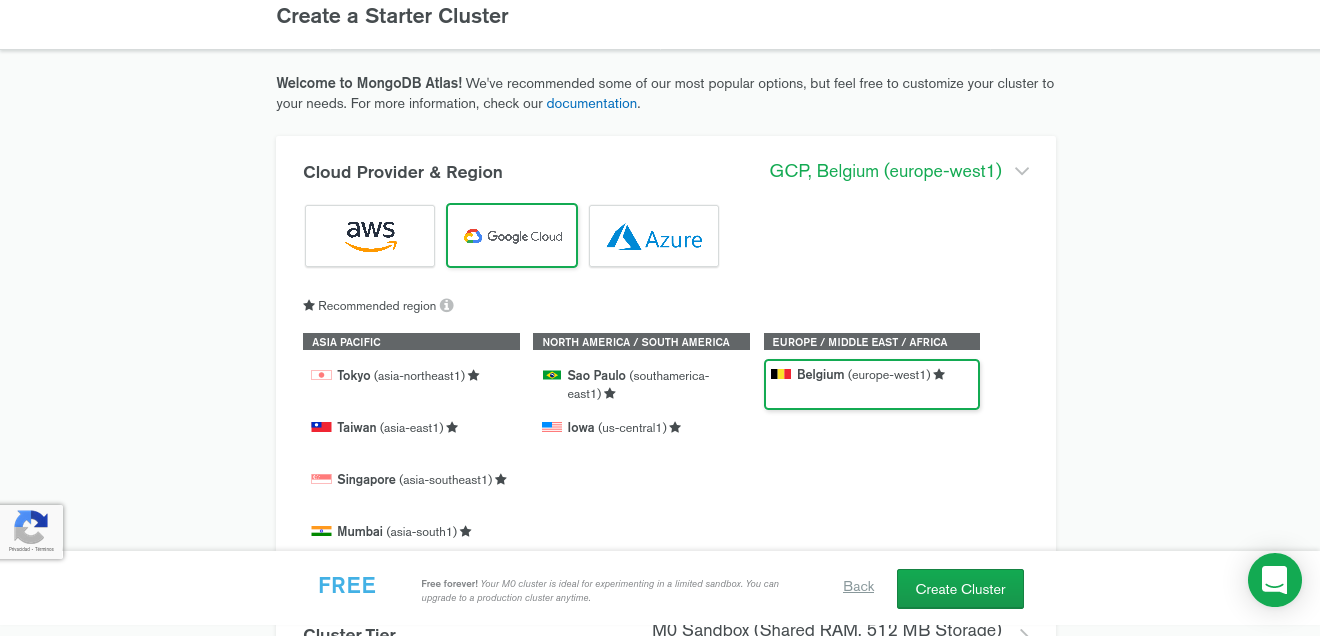
\includegraphics[scale=0.3]{1.png}
	\end{figure}
	\item Seleccionamos ADF Fusion Web Application $\rightarrow$ Ok
	\item Ya empezamos a darle nombre a nuestra aplicación: HRSystem. La ruta dejamos la que nos daba por defecto y Application Package Prefix: demo $\rightarrow$ Siguiente
	\pagebreak
	\begin{figure}[!h]
	  \centering
	    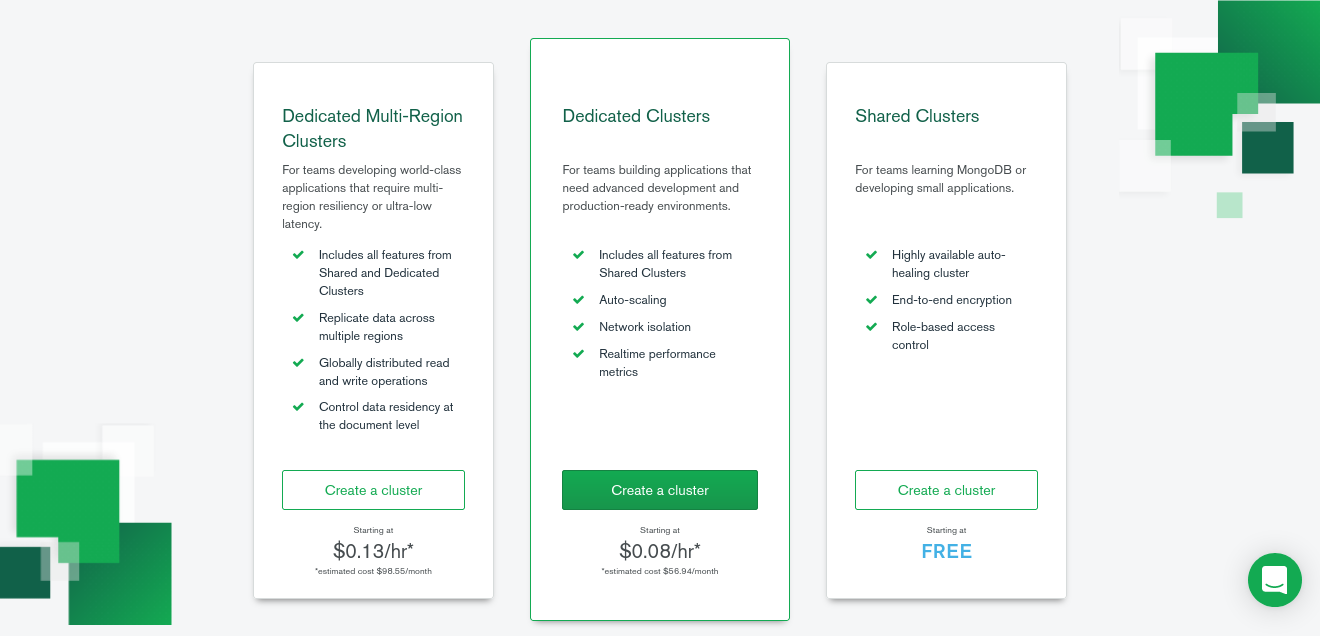
\includegraphics[scale=0.3]{2.png}
	\end{figure}
	\item En Project 1 Name nos aseguramos de que Project Name: Model $\rightarrow$ Siguiente
	\begin{figure}[!h]
	  \centering
	    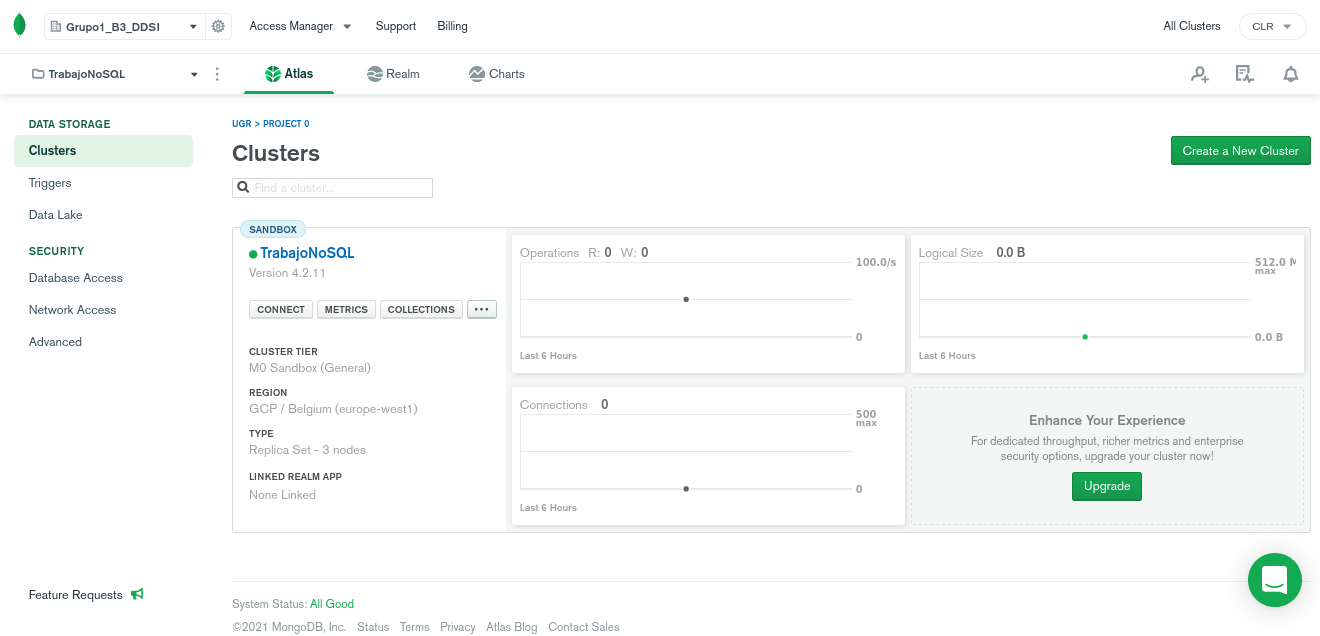
\includegraphics[scale=0.3]{3.png}
	\end{figure}
	\item En Project 1 Java Settings dejamos los valores predeterminados $\rightarrow$ Siguiente
	\pagebreak
	\begin{figure}[!h]
	  \centering
	    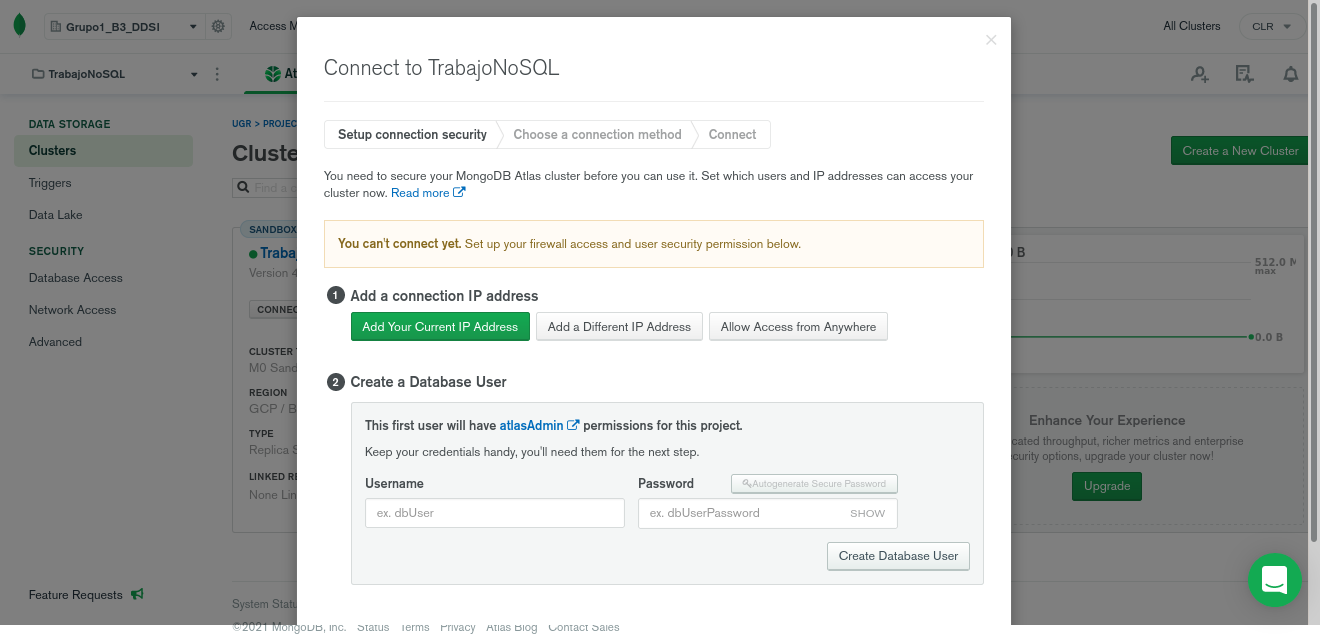
\includegraphics[scale=0.3]{4.png}
	\end{figure}
	\item En project 2 Name nos aseguramos de que Project Name: ViewController $\rightarrow$ Siguiente
	\begin{figure}[!h]
	  \centering
	    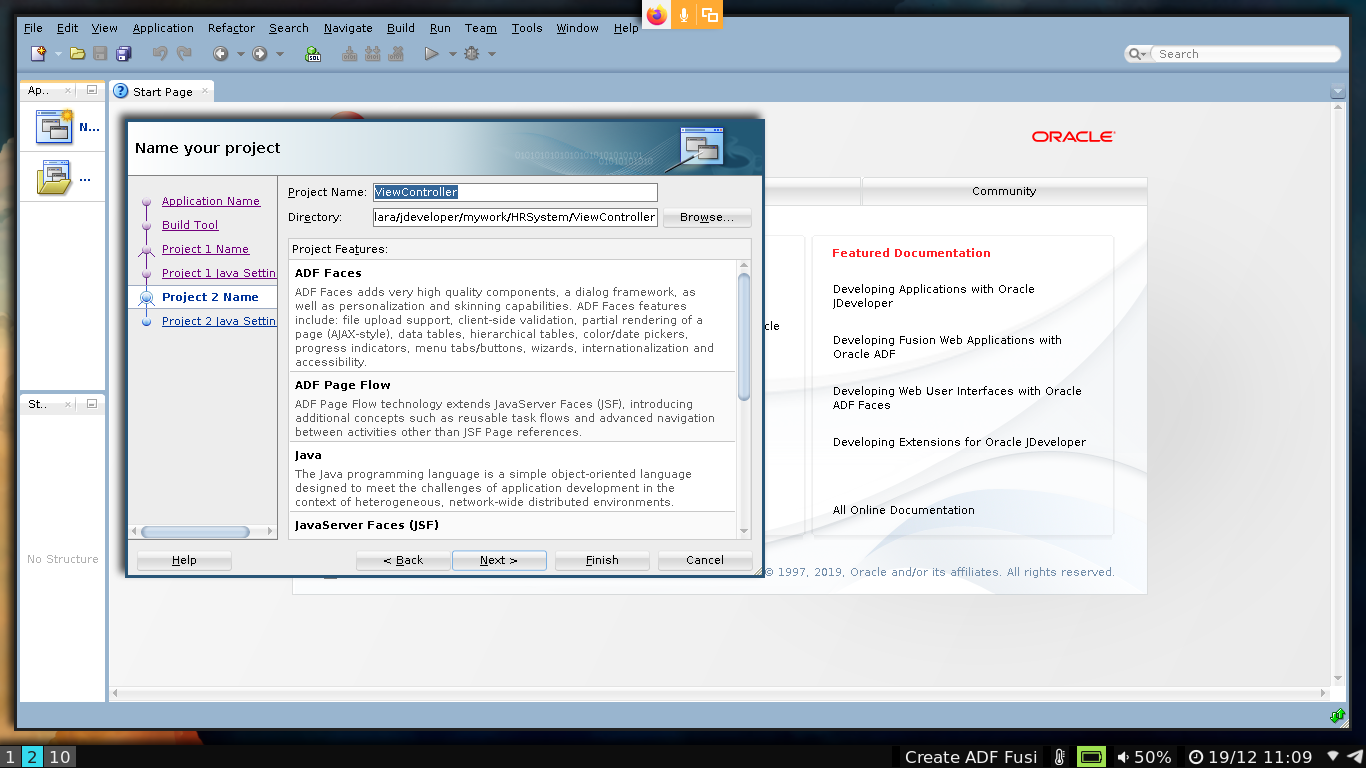
\includegraphics[scale=0.3]{5.png}
	\end{figure}
	\item Damos click en Finish y así creamos nuestra aplicación y proyectos Fusión Web.

\end{enumerate}

\pagebreak

\subsection{Desarrollar los servicios comerciales}
Nos conectaremos a nuestra base de datos y accederemos a las tablas
\begin{enumerate}
	\item Damos click en Connect to a Database.
	\item Damos click en Create a Database Connection.
	\item Rellenamos los campos como hacíamos en el seminario 2, conectados también a la VPN de la UGR $\rightarrow$ Ok
	\begin{enumerate}
		\item Connection Name: HRConn
		\item Connection Type: Oracle (JDBC)
		\item Username: nuestro DNI con la primera letra una ``x''
		\item Password: la misma que username
		\item Hostname: oracle0.ugr.es
		\item Service name: practbd.oracle0.ugr.es
		\item JDBC Port: 1521
	\end{enumerate}
	\begin{figure}[!h]
	  \centering
	    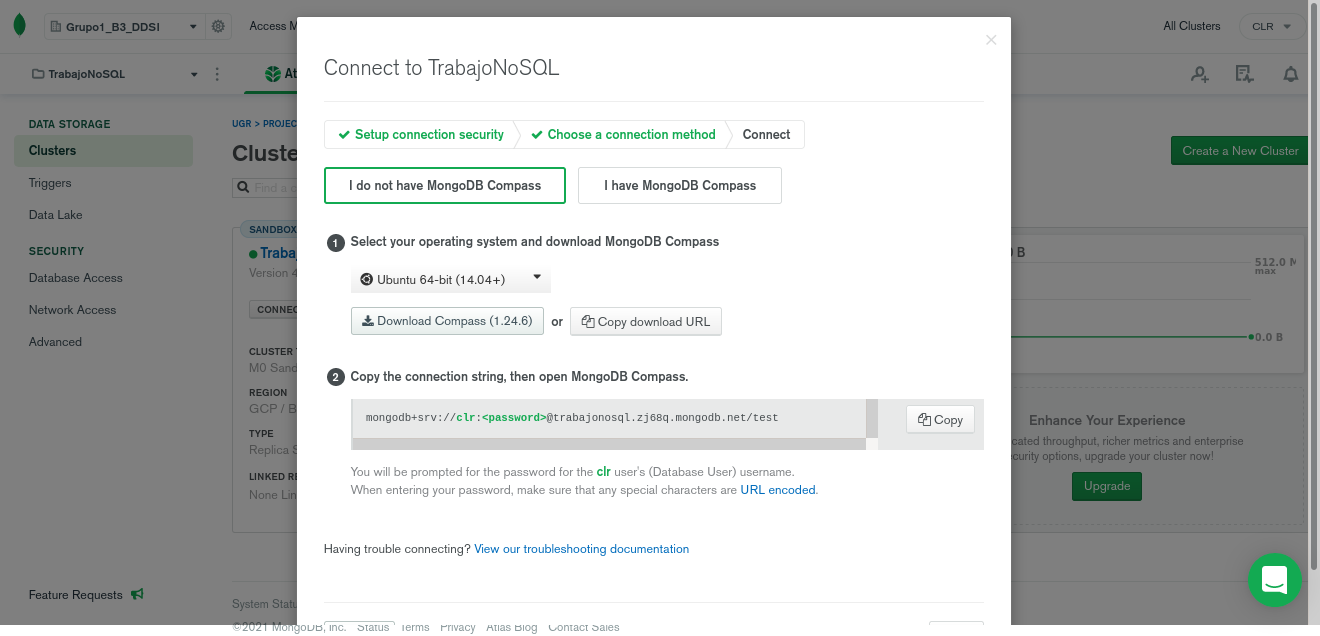
\includegraphics[scale=0.3]{6.png}
	\end{figure}
	\pagebreak
	\item Marcamos el estado de Connect to a Database > Done
	\begin{figure}[!h]
	  \centering
	    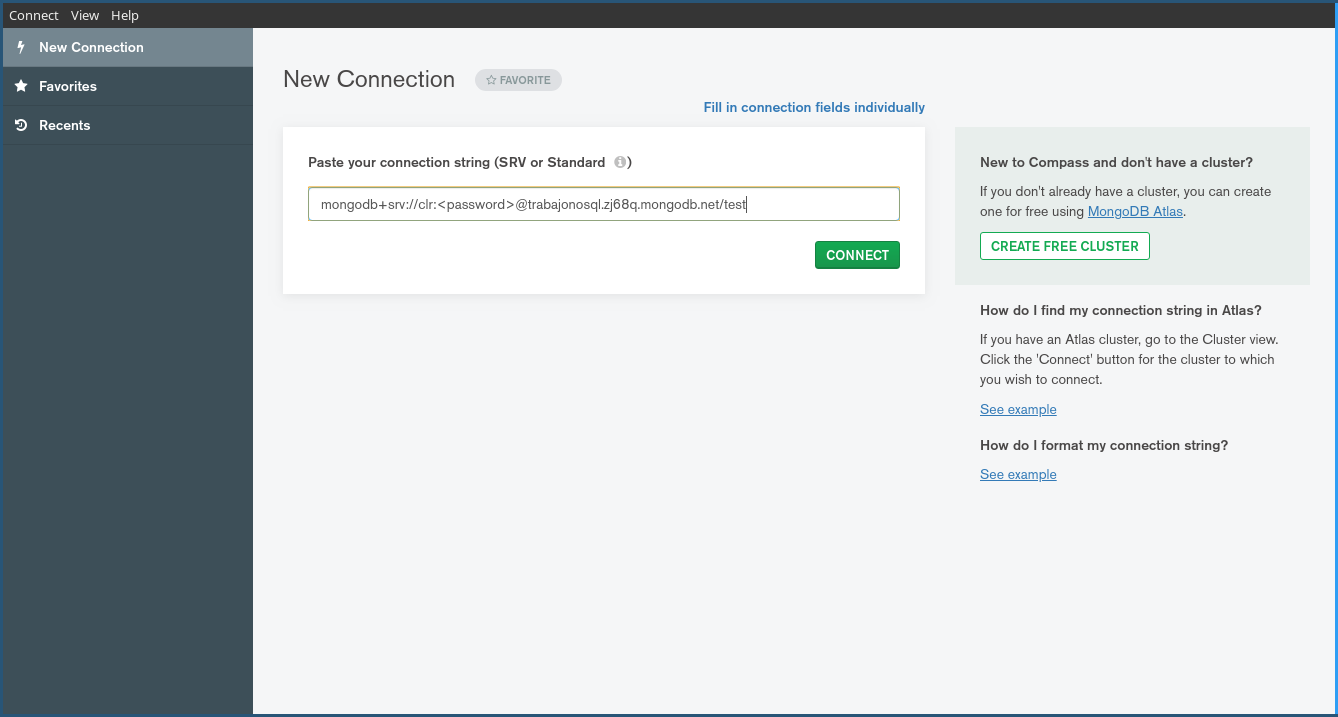
\includegraphics[scale=0.3]{7.png}
	\end{figure}
	\item Seleccionamos Build Business Services para expandirlos y hacemos click en Go to Substeps
	\item Pulsamos el primer paso: Create Entity Objects and Associations
	\begin{figure}[!h]
	  \centering
	    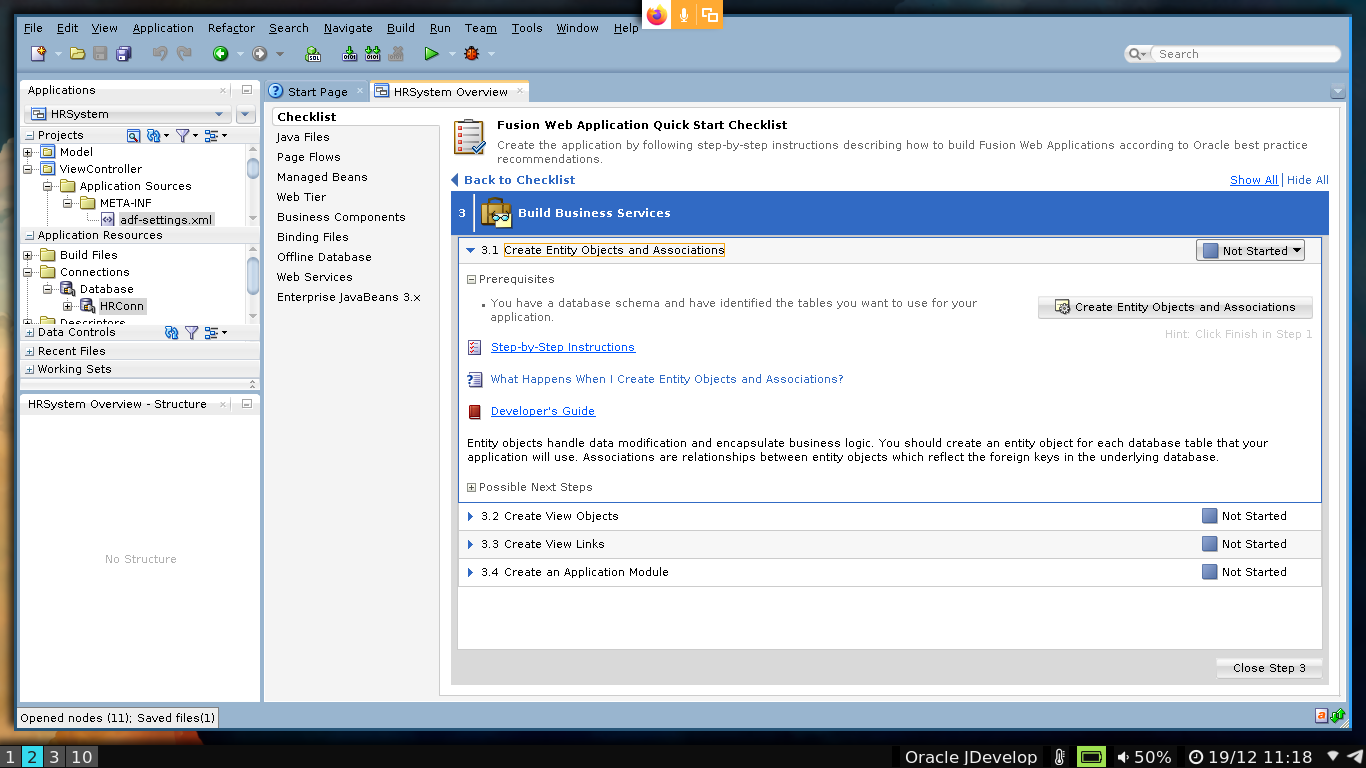
\includegraphics[scale=0.3]{8.png}
	\end{figure}
	\item Seleccionamos el proyecto Model $\rightarrow$ Ok
	\pagebreak
	\begin{figure}[!h]
	  \centering
	    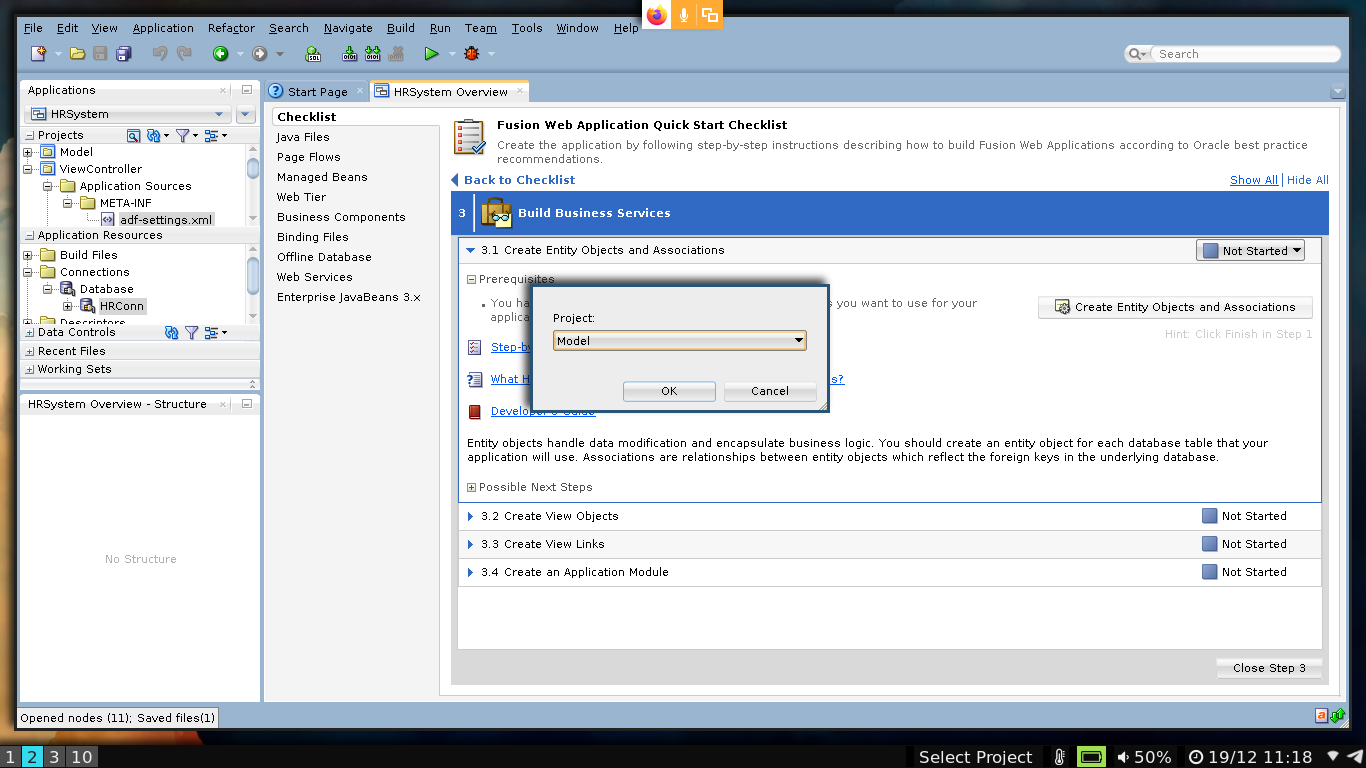
\includegraphics[scale=0.3]{9.png}
	\end{figure}
	\item Se nos abre la siguiente ventana y empezamos a crear ``Business Components'' a partir de las tablas. Seleccionamos, dentro de Entity Objects, el botón Query para ver las tablas disponibles.
	\begin{figure}[!h]
	  \centering
	    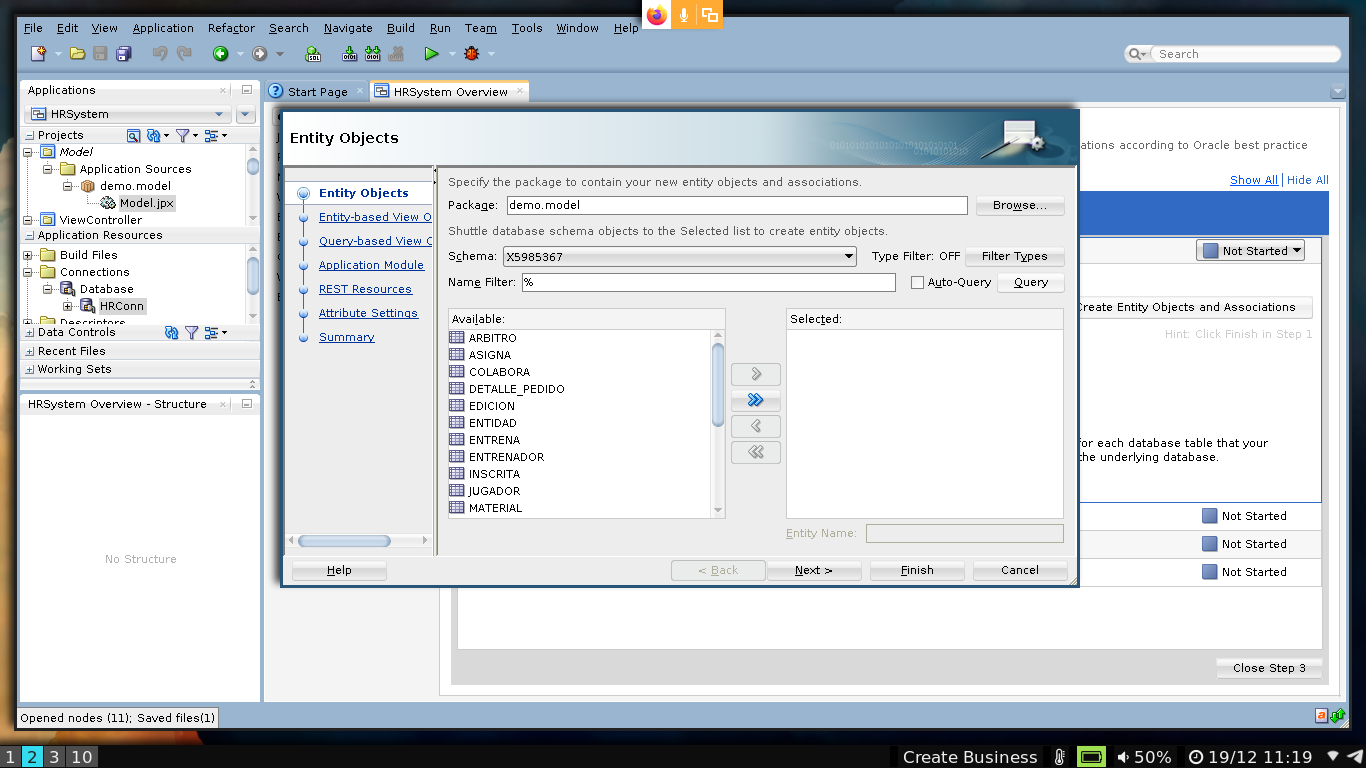
\includegraphics[scale=0.3]{10.png}
	\end{figure}
	\item Seleccionamos las tablas Detalle\_pedido, Pedido y Stock y hacemos click en la flecha hacia la derecha. Con este paso hemos conseguido crear objetos de entidad que pueden ser actualizados basados en las tablas seleccionadas.
	\pagebreak
	\begin{figure}[!h]
	  \centering
	    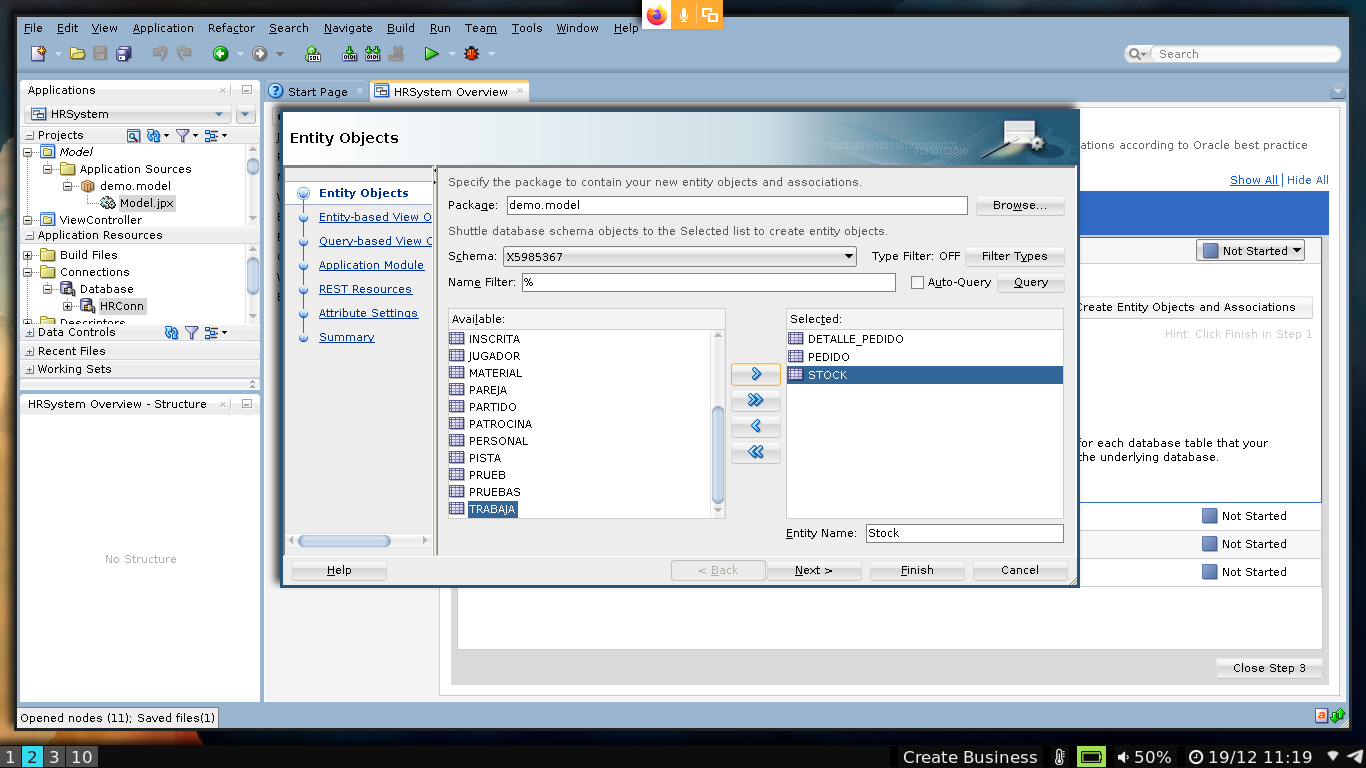
\includegraphics[scale=0.3]{11.png}
	\end{figure}
	\item En el siguiente paso (Entity-based View Objects) movemos las tres tablas a la sección ``Seleccionado'' $\rightarrow$ Siguiente
	\item En los dos siguientes pasos dejamos los datos por defecto y finalizamos.
	\begin{figure}[!h]
	  \centering
	    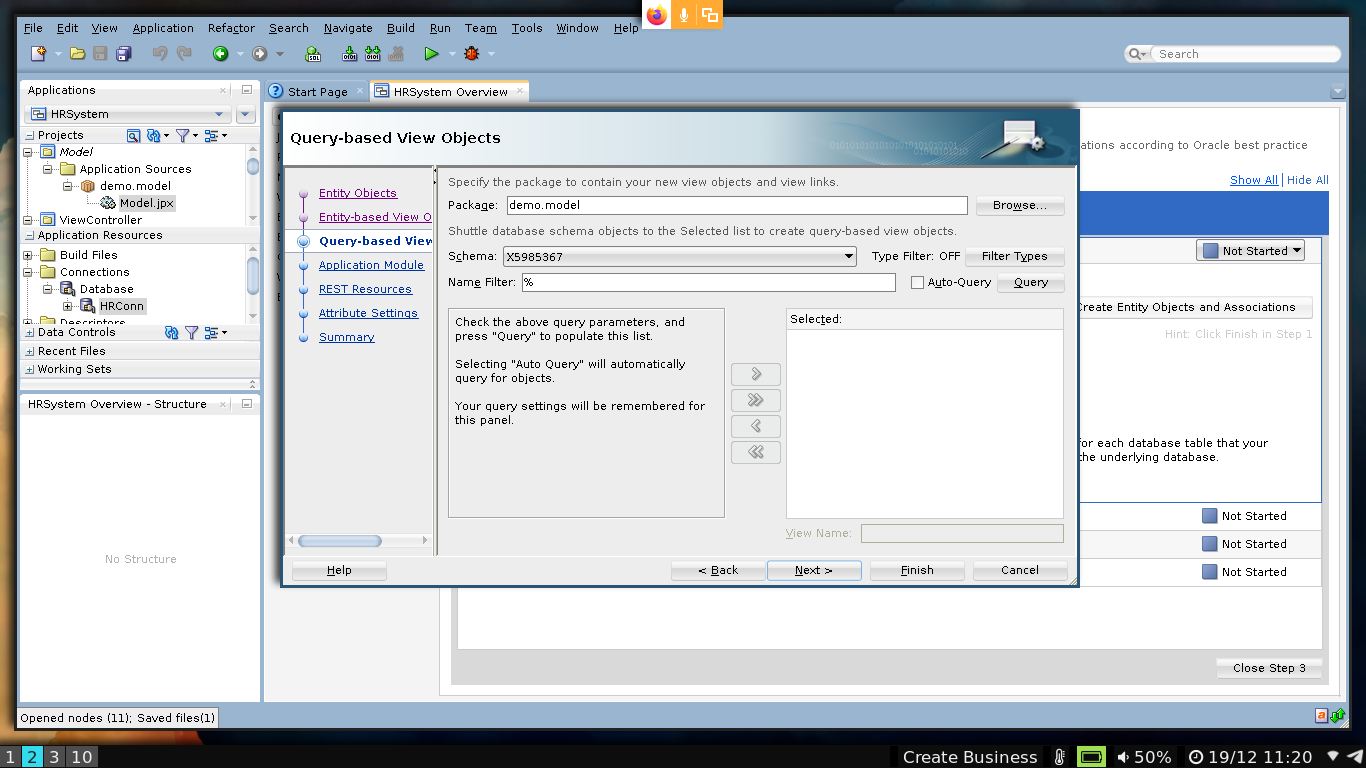
\includegraphics[scale=0.3]{12.png}
	\end{figure}
	\pagebreak
	\begin{figure}[!h]
	  \centering
	    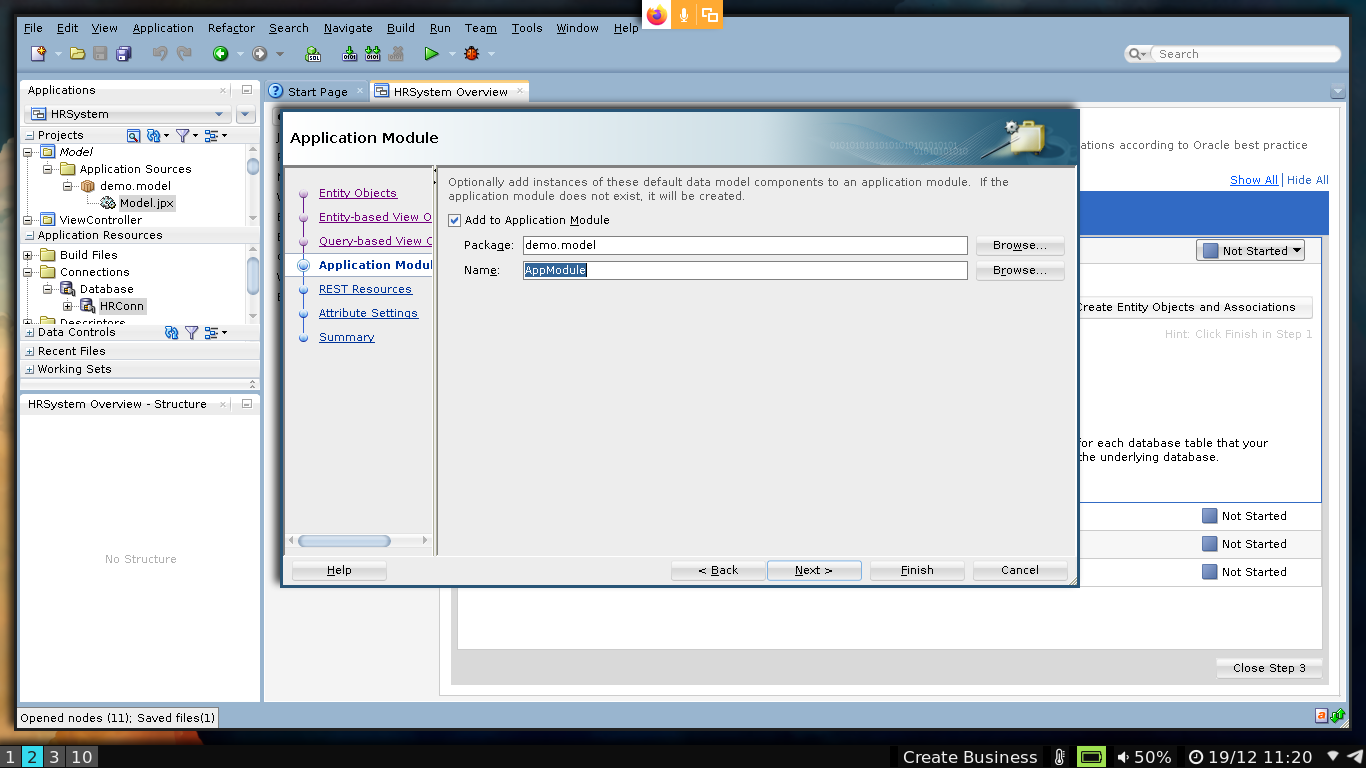
\includegraphics[scale=0.3]{13.png}
	\end{figure}
	\begin{figure}[!h]
	  \centering
	    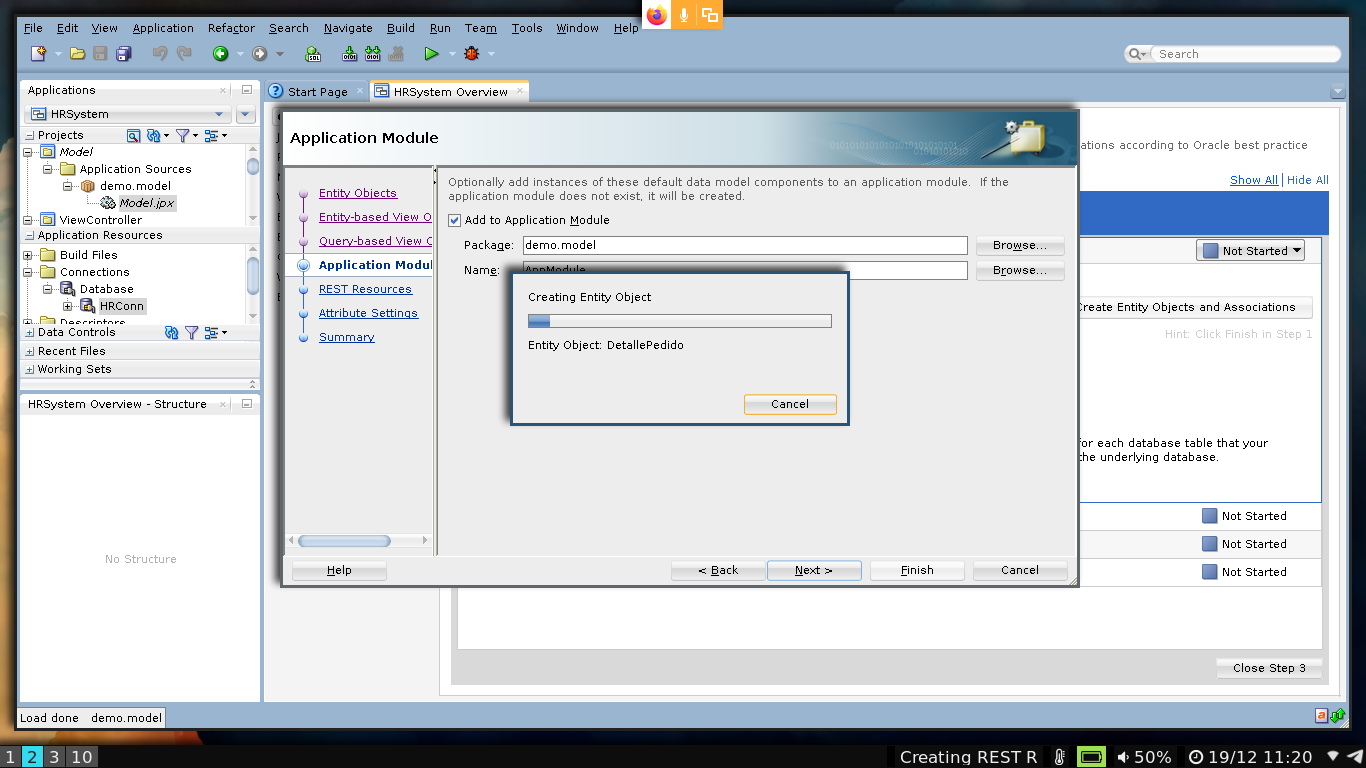
\includegraphics[scale=0.3]{14.png}
	\end{figure}
	\item Ahora, ya podemos poner en estado ``Done'' el paso ``Create Entity Objects and Associations''
	\pagebreak
	\begin{figure}[!h]
	  \centering
	    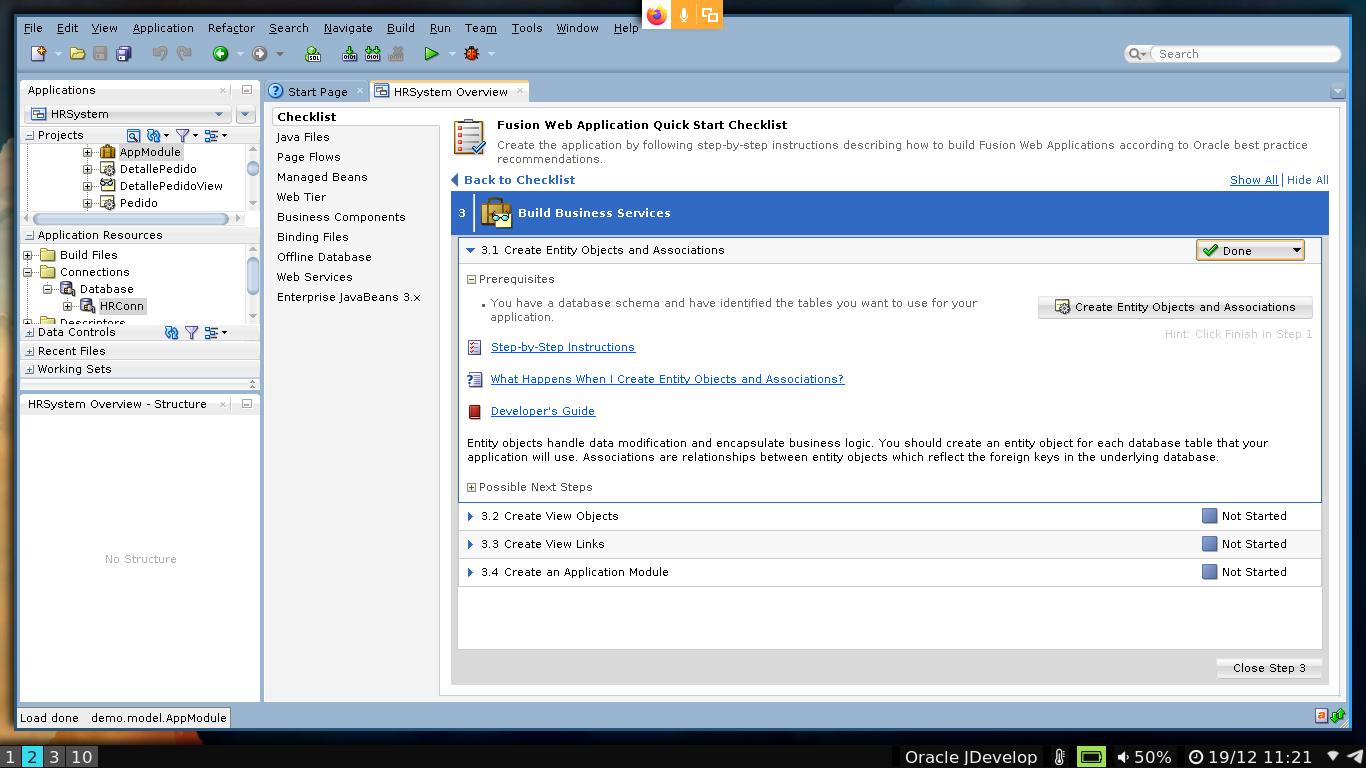
\includegraphics[scale=0.3]{15.png}
	\end{figure}
	\item Cerramos el paso 3.
	\item Ponemos el estado de ``Build Business Services'' a ``Done''
	\begin{figure}[!h]
	  \centering
	    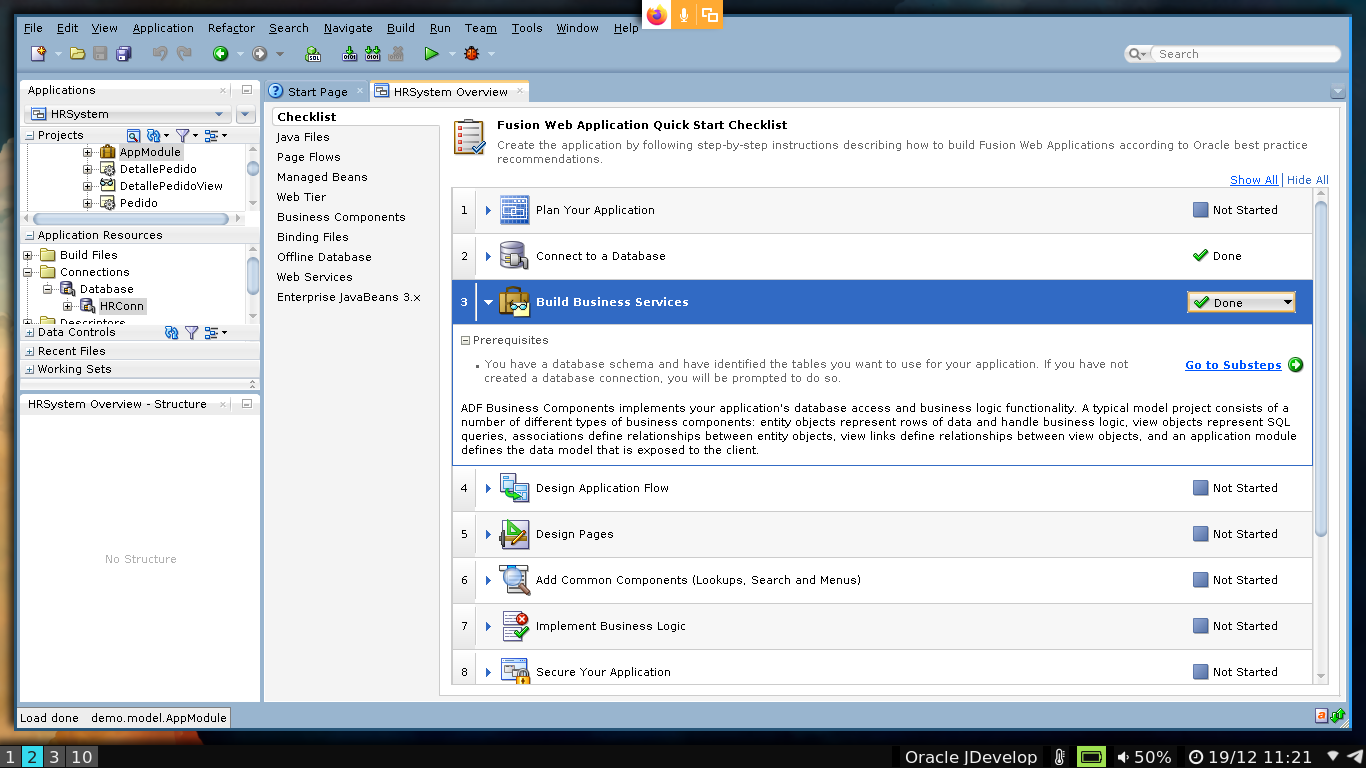
\includegraphics[scale=0.3]{16.png}
	\end{figure}
	\item A continuación, en la ventana de la derecha, donde pone ``Applications'', en la sección ``AppModule'' hacemos click derecho $\rightarrow$ Run para probar lo que acabamos de crear. Nos sale una ventana para ver en qué carpeta lo guardamos:
	\pagebreak
	\begin{figure}[!h]
	  \centering
	    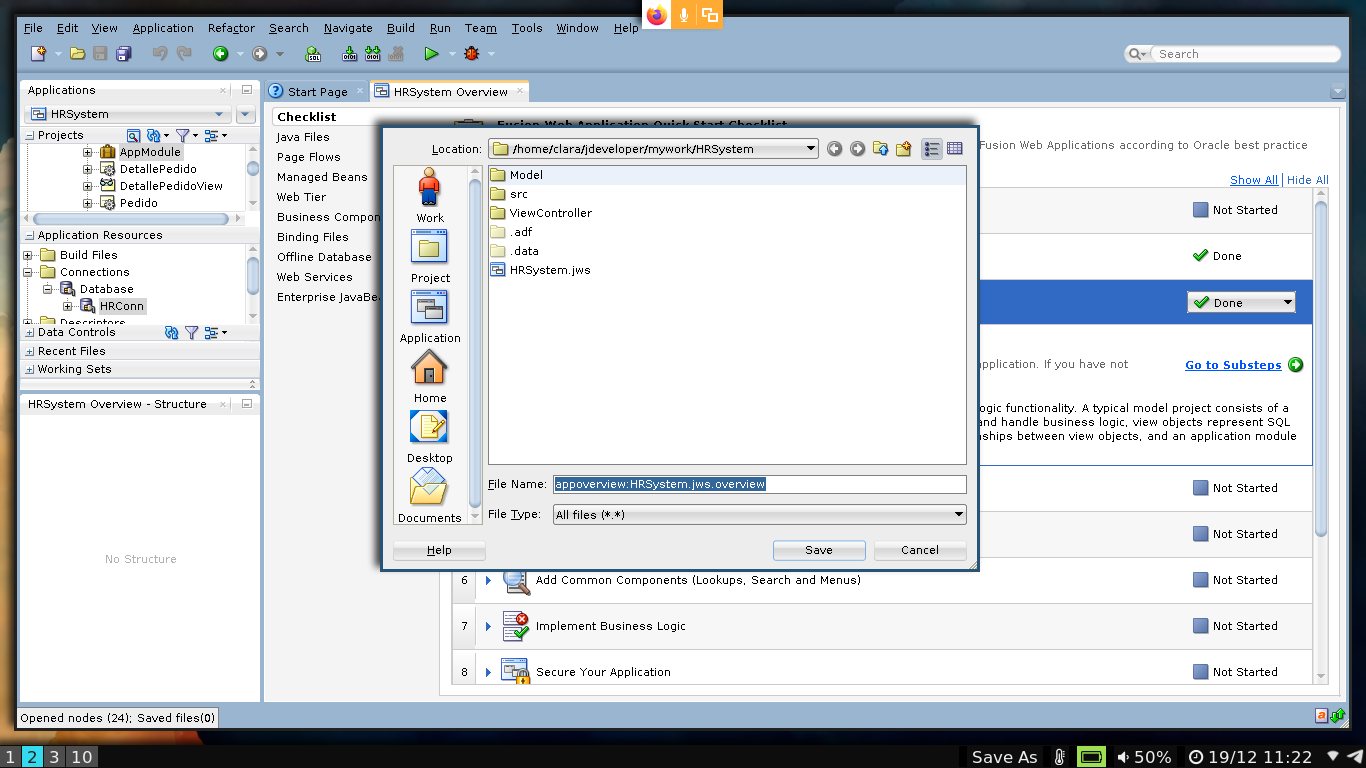
\includegraphics[scale=0.3]{17.png}
	\end{figure}
	\item Hacemos doble click en StockView2 para ver sus datos. Haremos un filtro para ver la cantidad de productos con el código 3:
	\begin{figure}[!h]
	  \centering
	    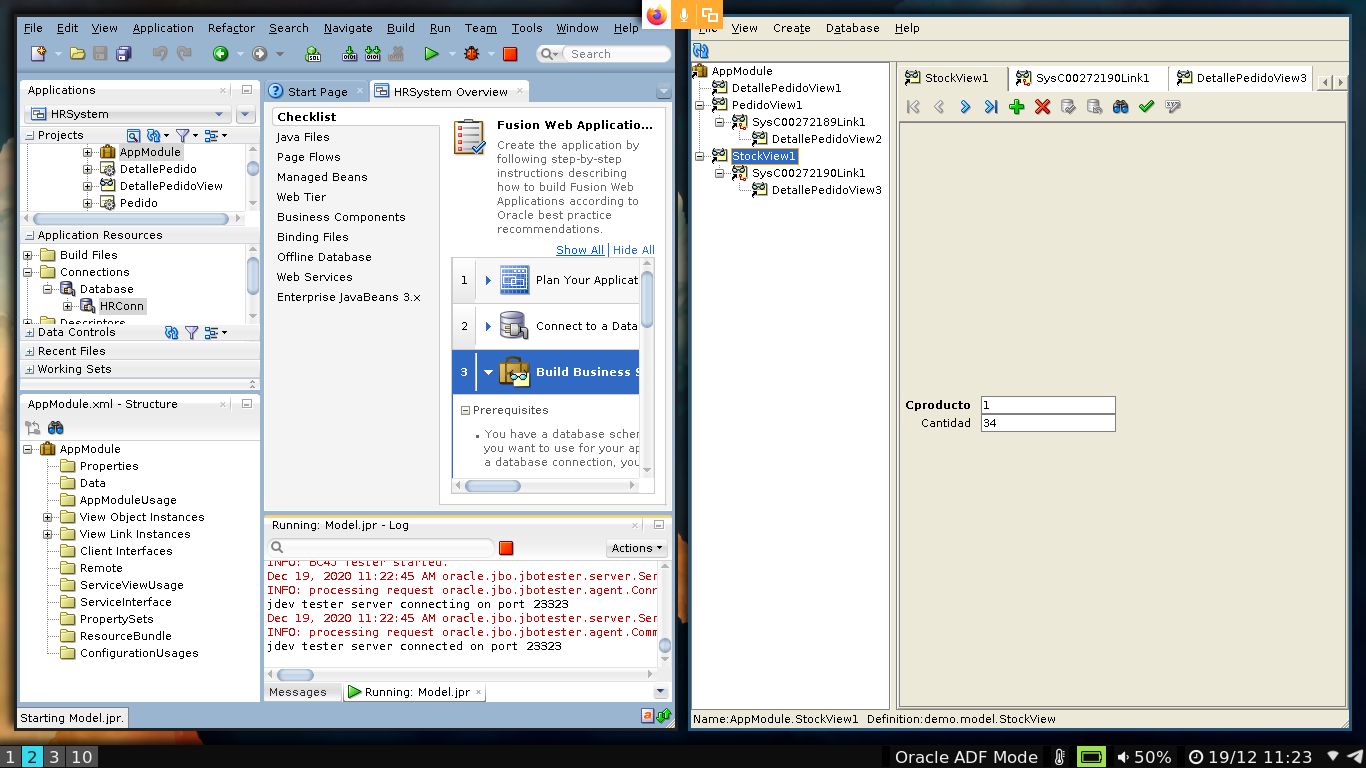
\includegraphics[scale=0.3]{18.png}
	\end{figure}
	\pagebreak
	\begin{figure}[!h]
	  \centering
	    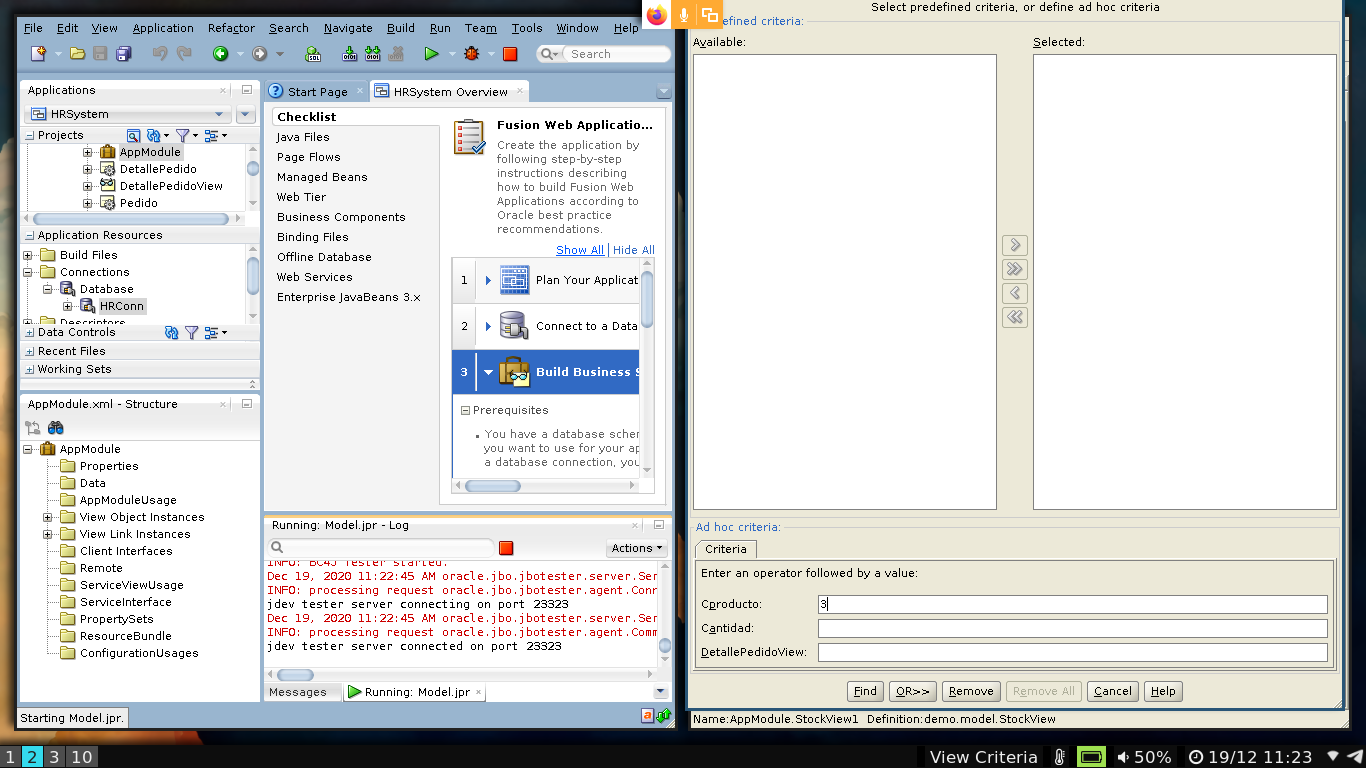
\includegraphics[scale=0.3]{19.png}
	\end{figure}
	\item Hay que tener en cuenta que para acceder a todos los datos de nuevo, hay que eliminar los parámetros de filtro que hemos metido.
	\item File $\rightarrow$ Save All.
\end{enumerate}

\subsection{Desarrollar una página con Java Server Faces}
JavaServer Faces es un framework que nos permite simplificar el desarrollo de interfaces de usuario para aplicaciones Java EE. Para acceder a los \textit{business components} que hemos creado anteriormente vamos a crear una JSF.
\begin{enumerate}
	\item Hacemos click derecho sobre \texttt{ViewController $\rightarrow$ New $\rightarrow$ Page}. La parte web de la aplicación se desarrolla por separado en un proyecto que es el ViewController, creado cuando creamos la Fusion Web application. De esta forma, si separamos la Model layer y la interfaz de usuario separadas, la capa de servicio será reutilizable.
	\begin{figure}[!h]
	  \centering
	    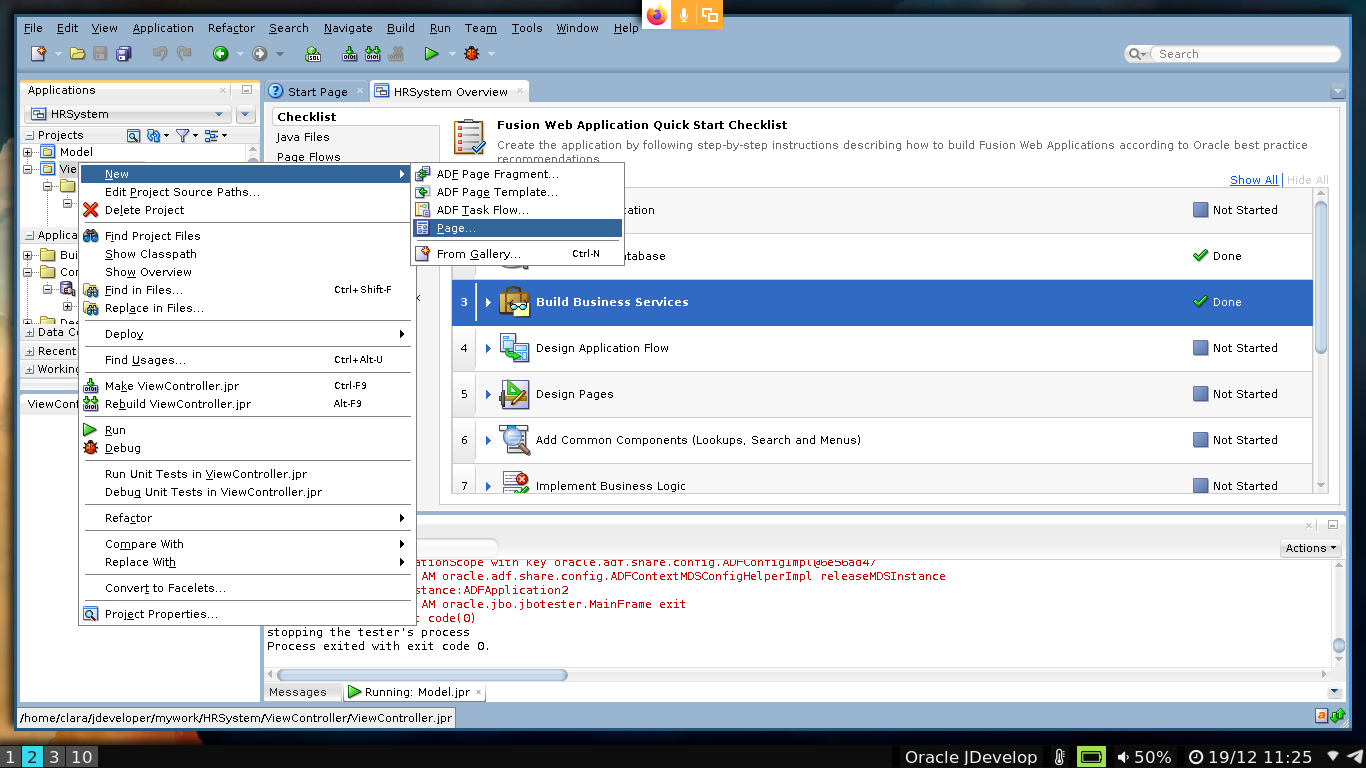
\includegraphics[scale=0.3]{20.png}
	\end{figure}
	\item En el panel que nos aparece le pone como nombre al fichero HR.jsf y el tipo de documento lo establecemos a ``Facelets''. Para obtener la plantilla de nuestra página seleccionamos ``Reference ADF Page Template''. A continuación seleccionamos ``Tablet First Template'' y hacemos click sobre OK.
	\begin{figure}[!h]
	  \centering
	    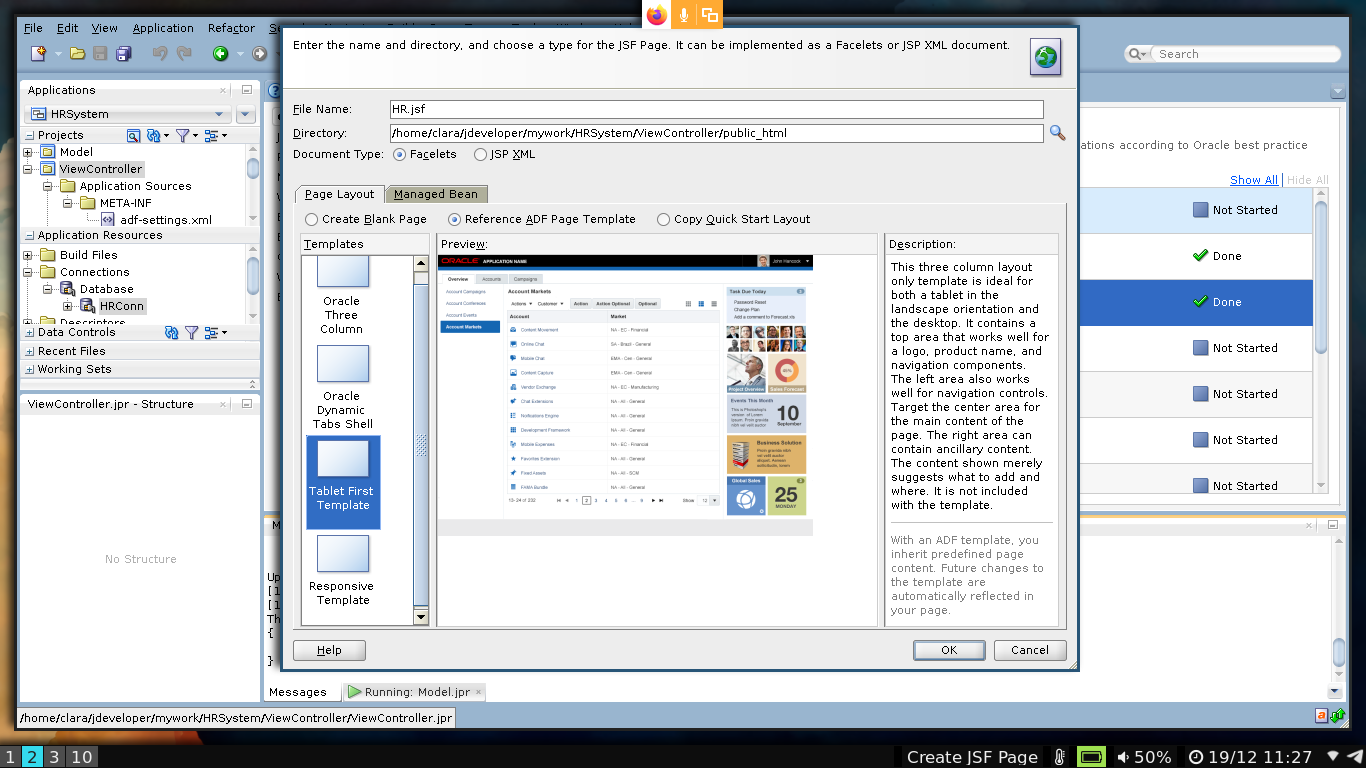
\includegraphics[scale=0.3]{21.png}
	\end{figure}
	\item Por defecto, en el centro vamos a tener el editor visual de la página, abajo a la izquierda el formato estructurado y abajo a la derecha las propiedades del ítem seleccionado.
	\begin{figure}[!h]
	  \centering
	    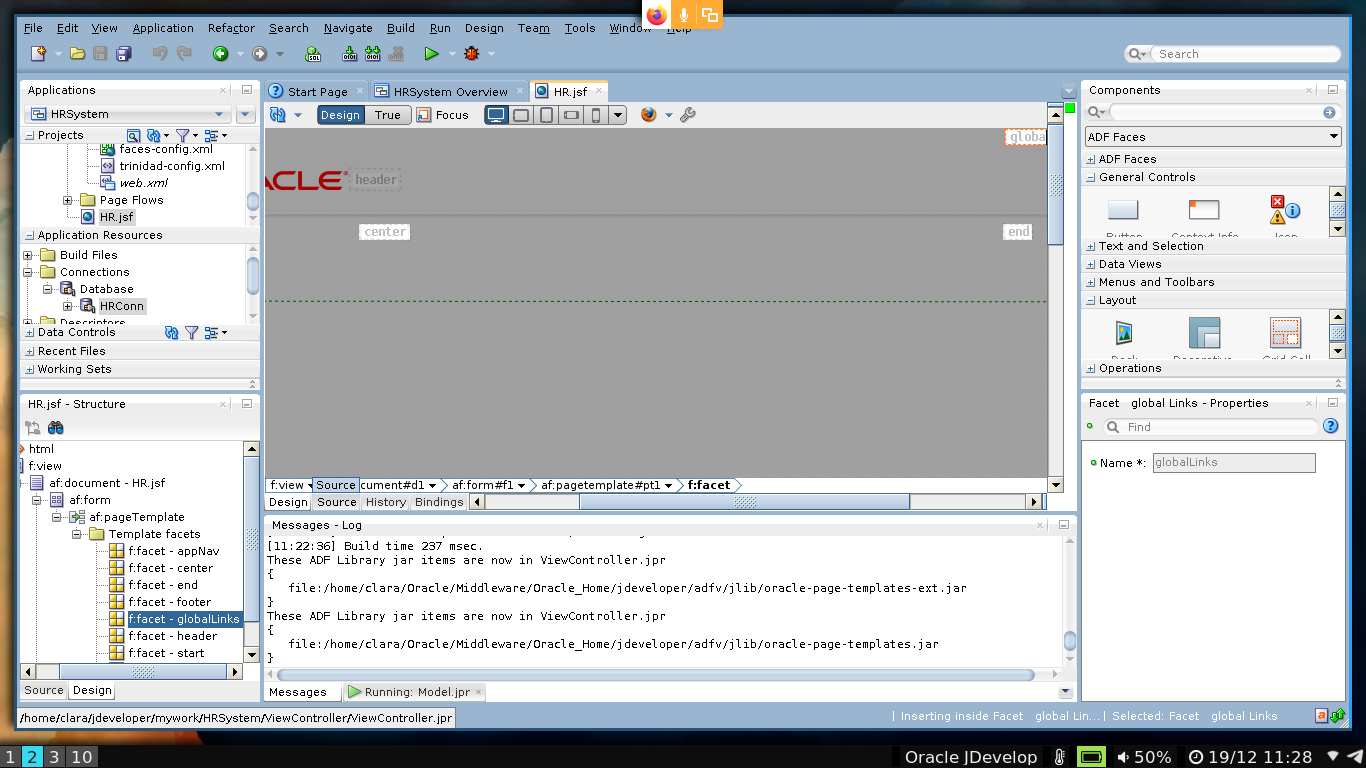
\includegraphics[scale=0.3]{22.png}
	\end{figure}
	\pagebreak
	\begin{figure}[!h]
	  \centering
	    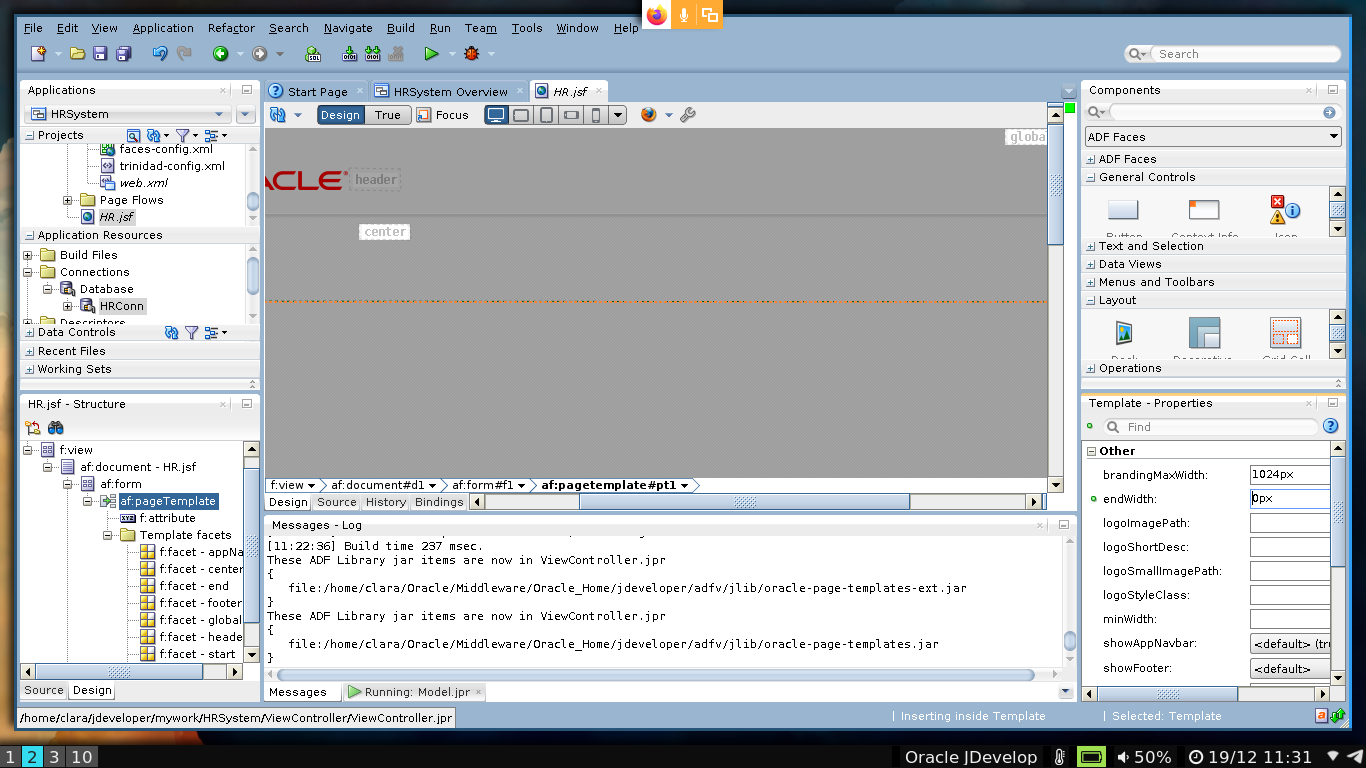
\includegraphics[scale=0.3]{23.png}
	\end{figure}
	\item Nos vamos abajo a la izquierda y expandimos \texttt{f:view $\rightarrow$ af:document-HR.jsf $\rightarrow$ af.form} y seleccionamos \texttt{af:pageTemplate} y abajo a la derecha ponemos endWith a 0px.
	\item Para añadir datos a la página usamos la ventana de ``Data Controls''. Expandimos abajo a la izquierda ``Template facets'', que es donde los datos serán mostrados en la página.  Hacemos click en DetallePedidoView1 y lo arrastramos hacia f:facet-start. Se nos mostrará un menú donde seleccionamos \texttt{Table/List View $\rightarrow$ ADF List View}. De esta forma se nos abrirá una ventana donde hemos de seleccionar la opción de Panel Grid Layout y hacemos click en Next.
	\begin{figure}[!h]
	  \centering
	    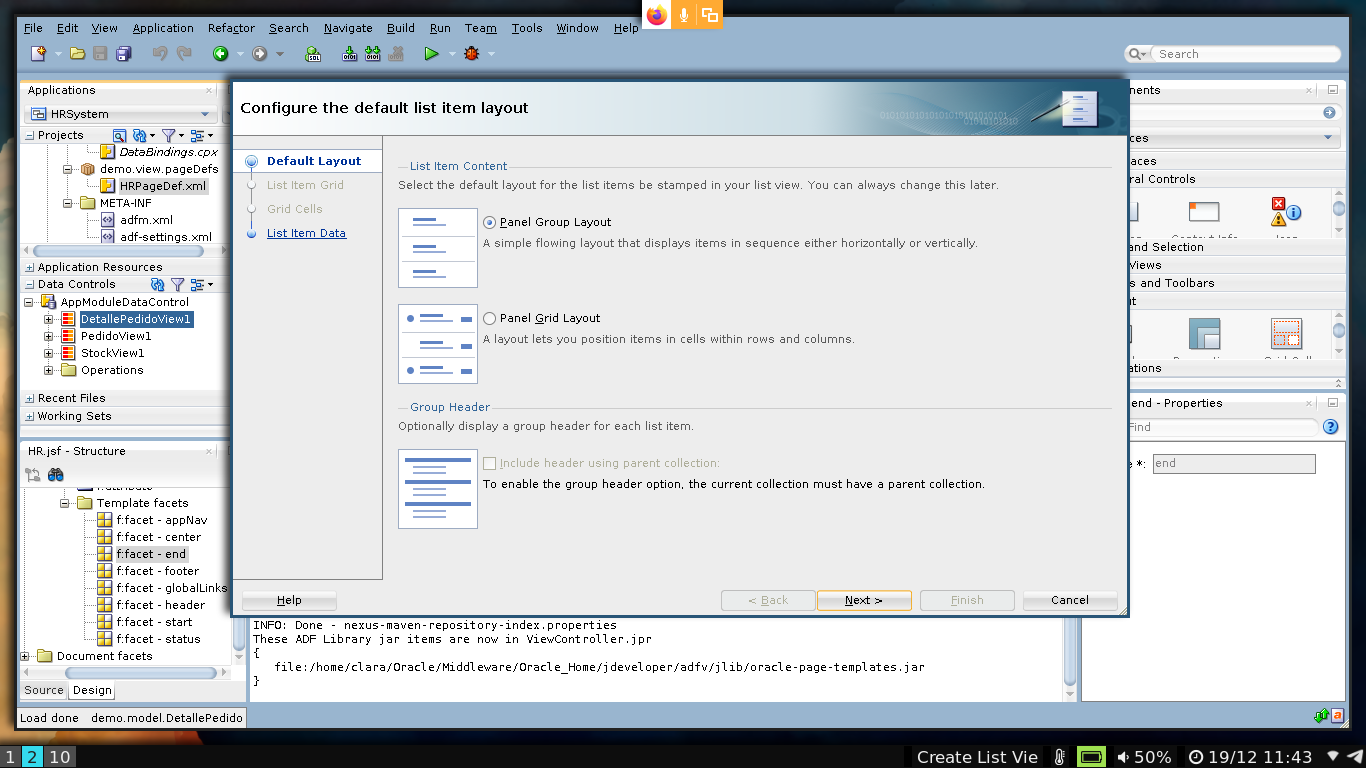
\includegraphics[scale=0.3]{24.png}
	\end{figure}
	\pagebreak
	\item Establecemos las columnas a 3 y las filas a 1
	\item Ponemos la columna 1 a 34\%, la 2 a 33\% y la 3 a 33\% de ancho. Estos eran los valores por defecto para tres columnas.
	\begin{figure}[!h]
	  \centering
	    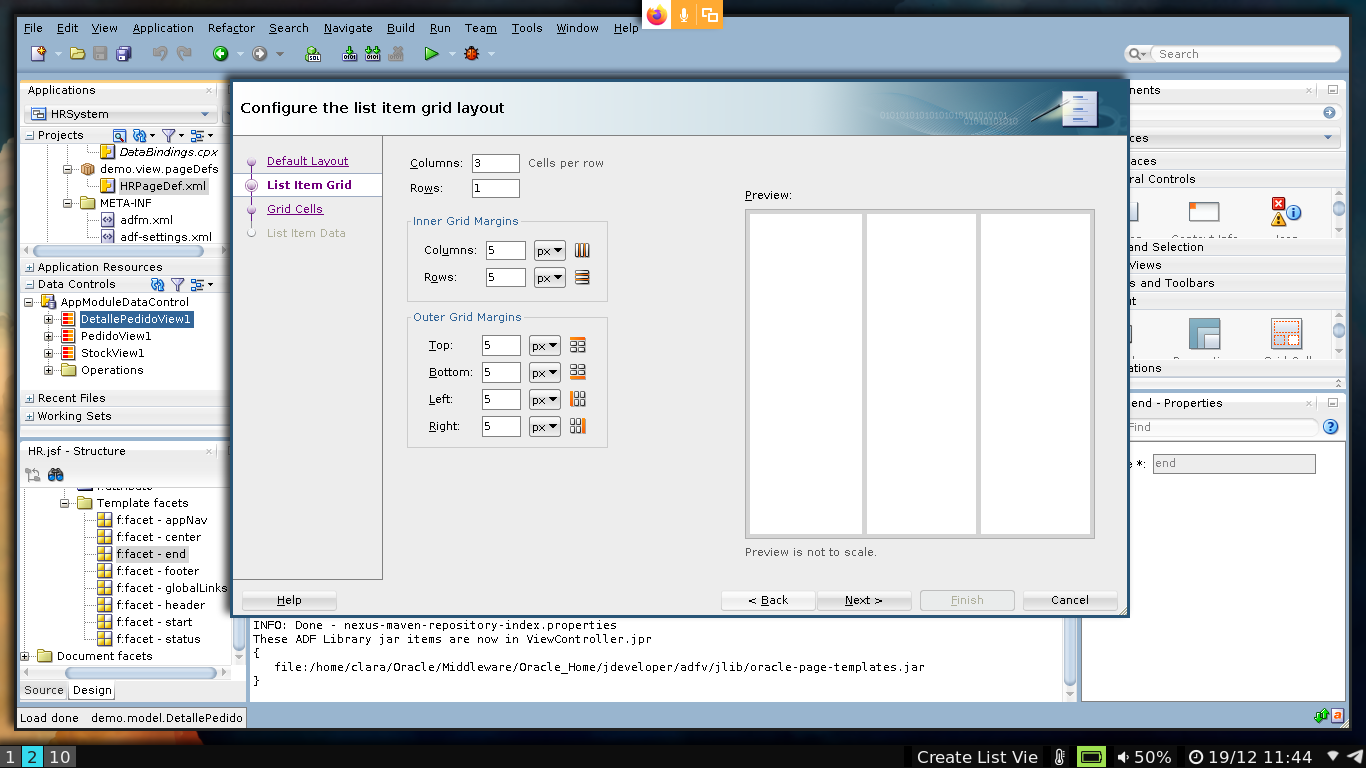
\includegraphics[scale=0.3]{25.png}
	\end{figure}
	\item Ponemos en la primera columna Cpedido, en la segunda Cproducto y en la tercera Cantidad y finalizamos.
	\begin{figure}[!h]
	  \centering
	    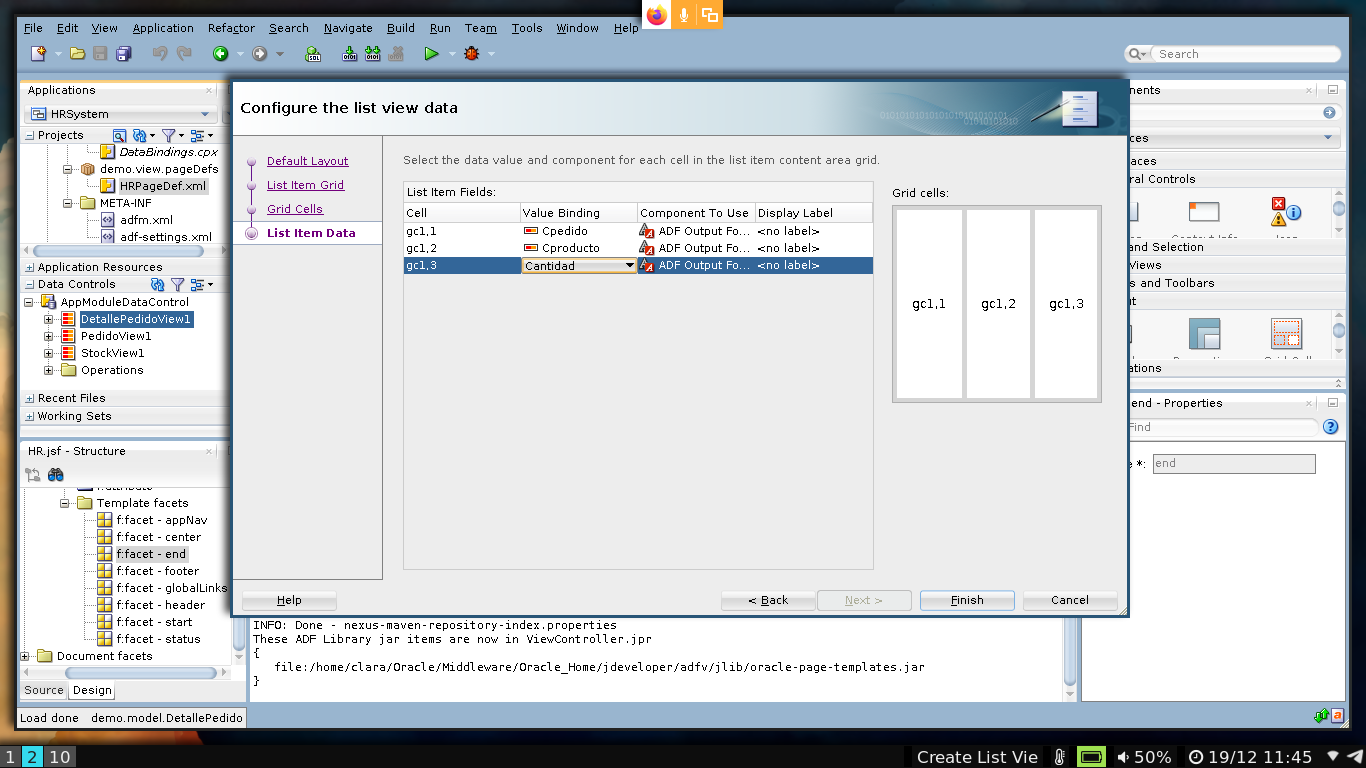
\includegraphics[scale=0.3]{26.png}
	\end{figure}
	\item Seleccionamos \texttt{af:listView} y en la ventana de Properties establecemos \texttt{Selection} a single
	\begin{figure}[!h]
	  \centering
	    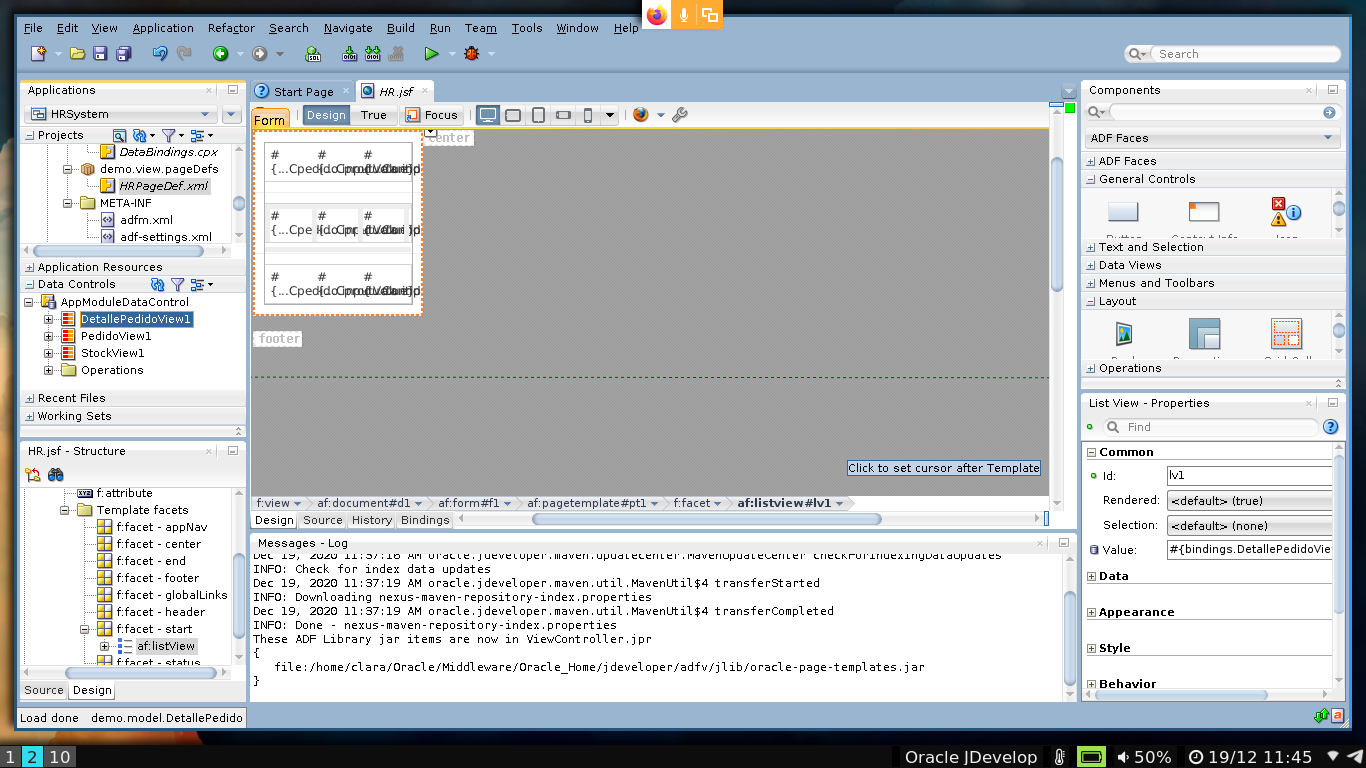
\includegraphics[scale=0.3]{27.png}
	\end{figure}
	\pagebreak
	\item En la misma ventana nos vamos a \texttt{Behaviour y hacemos} click sobre el engranaje de \texttt{SelectionListener}
	\begin{figure}[!h]
	  \centering
	    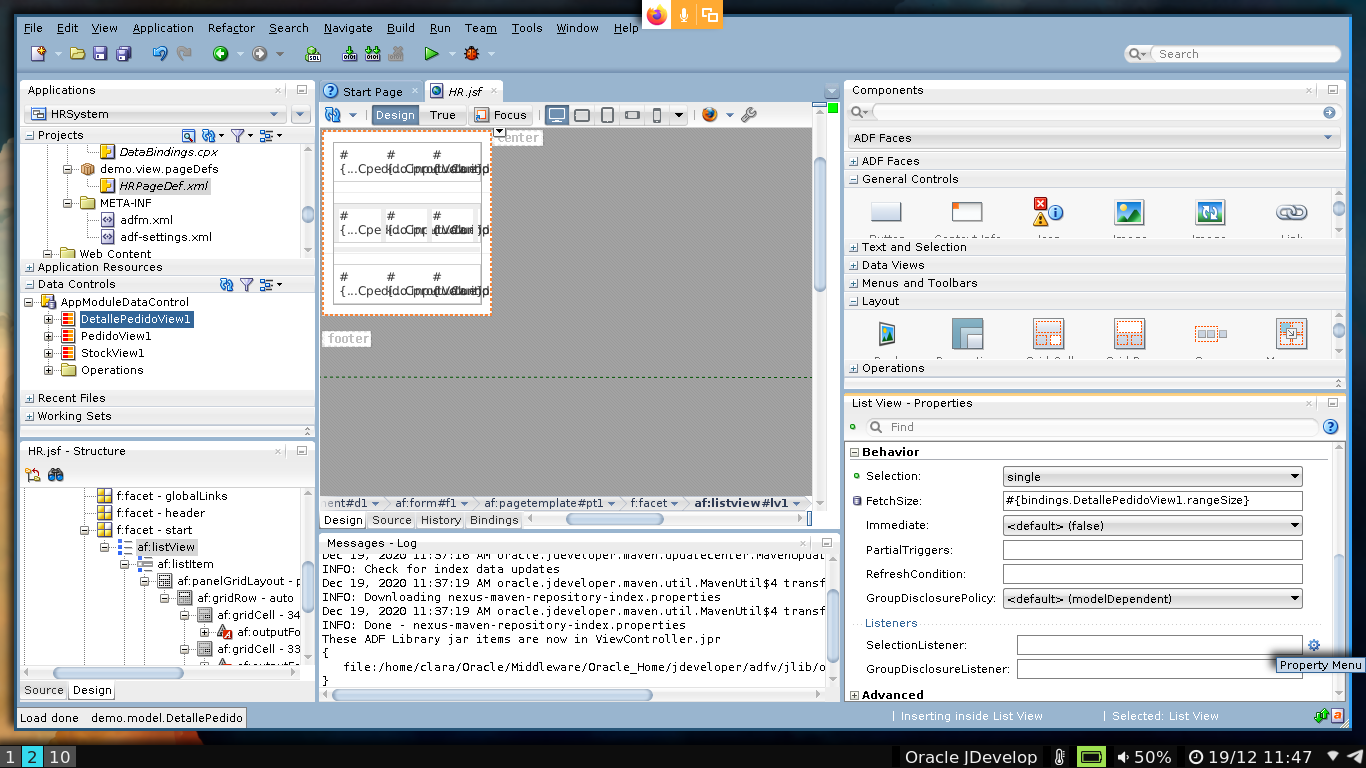
\includegraphics[scale=0.3]{28.png}
	\end{figure}
	\item En ``Method Expression Builder'' expandimos \texttt{ADF Bindings $\rightarrow$ bindings $\rightarrow$ DetallePedidoView1 $\rightarrow$ treeModel $\rightarrow$ makeCurrent} y hacemos click en OK
	\pagebreak
	\begin{figure}[!h]
	  \centering
	    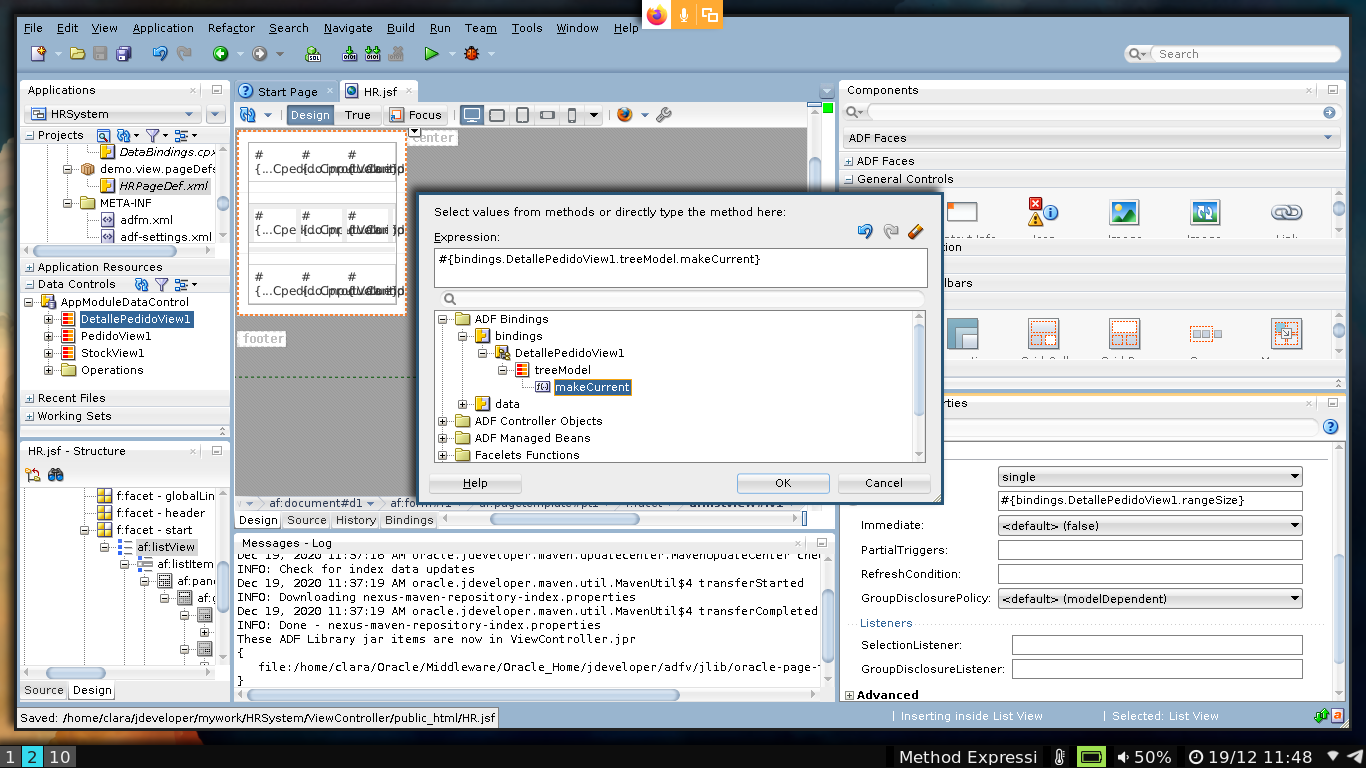
\includegraphics[scale=0.3]{29.png}
	\end{figure}
\end{enumerate}

\subsection{Testear la página desde un navegador}
Si es la primera vez que compilamos la página JDeveloper debemos de instalar WebLogic Server.
\begin{enumerate}
	\item  Para ello primero hemos de irnos a \texttt{Run $\rightarrow$ Start Server Instance}. Dejamos todo por defecto, sin contraseña.
	\begin{figure}[!h]
	  \centering
	    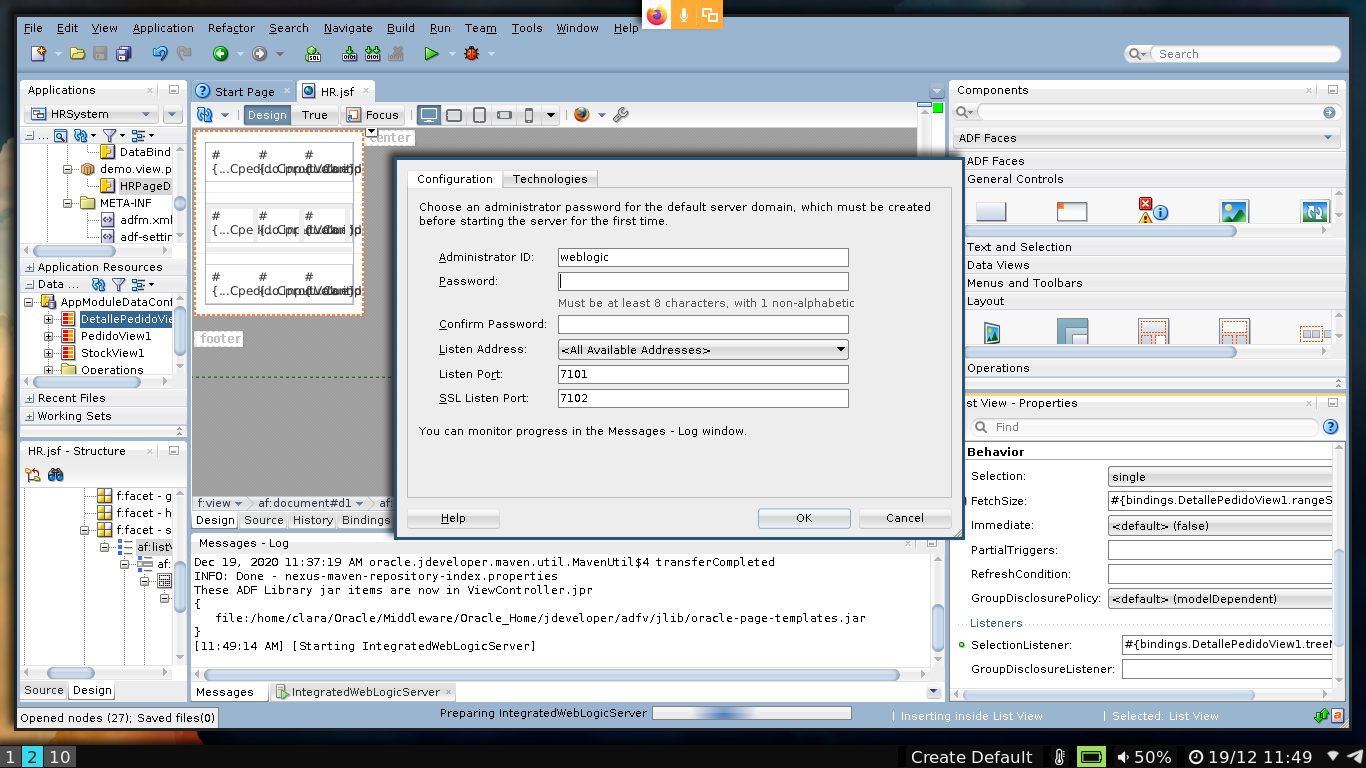
\includegraphics[scale=0.3]{30.png}
	\end{figure}
	\pagebreak
	\item Hacemos click derecho sobre el editor visual y seleccionamos \texttt{Run}.
	\begin{figure}[!h]
	  \centering
	    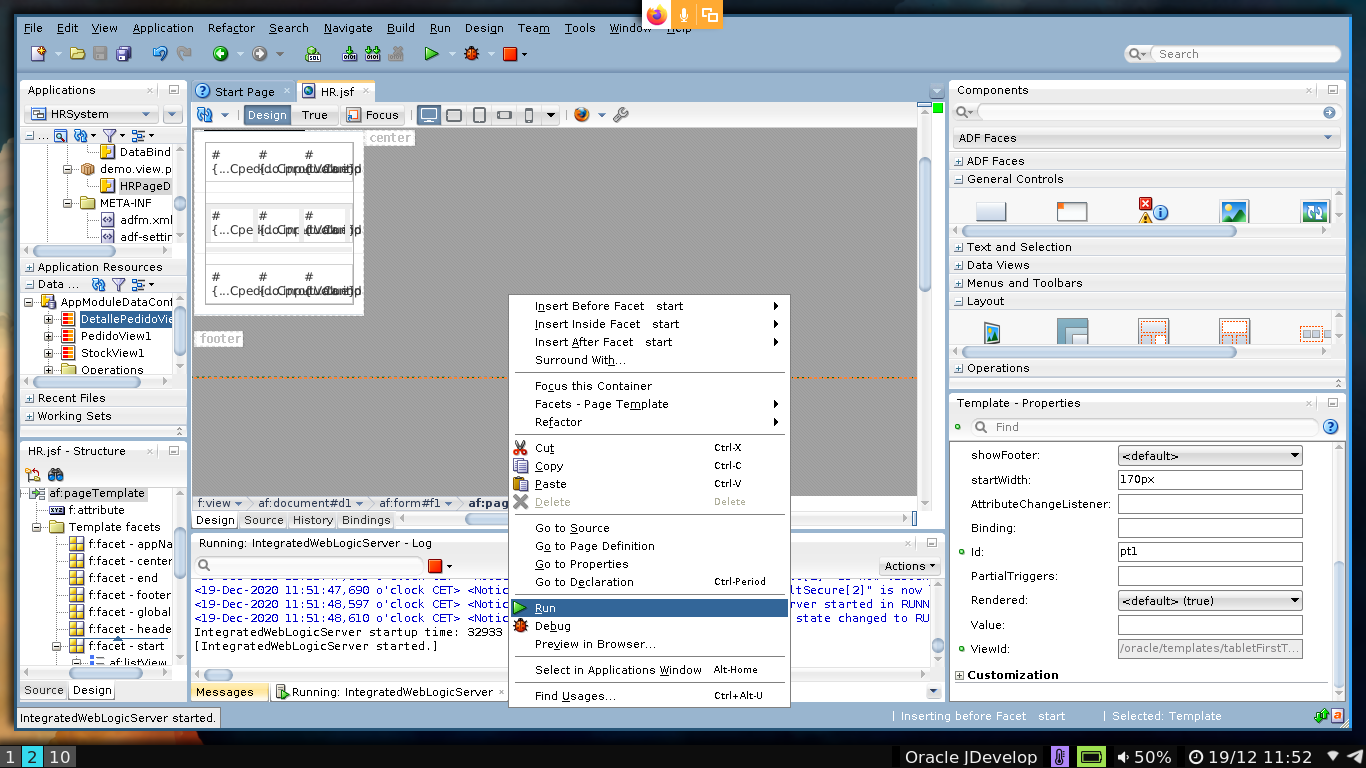
\includegraphics[scale=0.3]{31.png}
	\end{figure}

	Y se nos mostrará tras compilarlo en la ventana de abajo la URL local de nuestra página.
	\begin{figure}[!h]
	  \centering
	    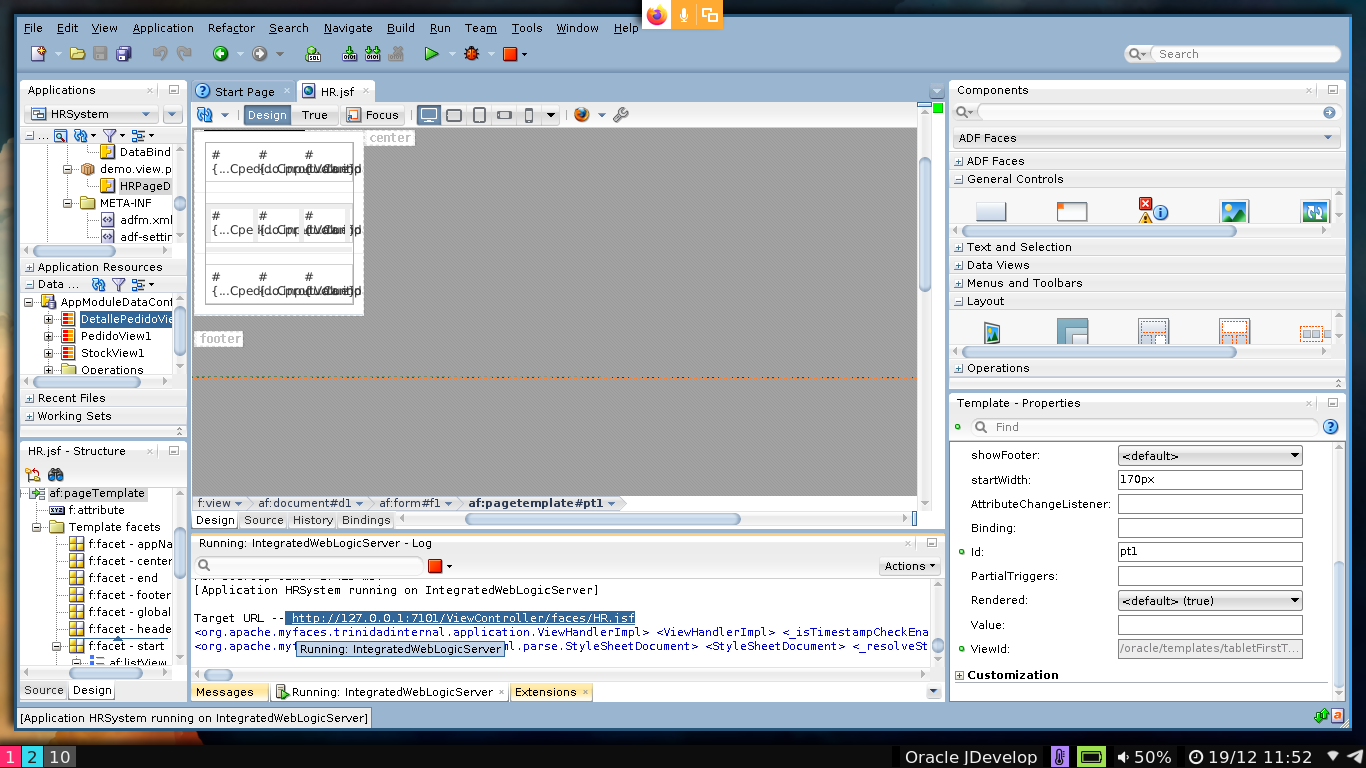
\includegraphics[scale=0.3]{32.png}
	\end{figure}
	\item Si la abrimos en un navegador veremos lo siguiente:
	\pagebreak
	\begin{figure}[!h]
	  \centering
	    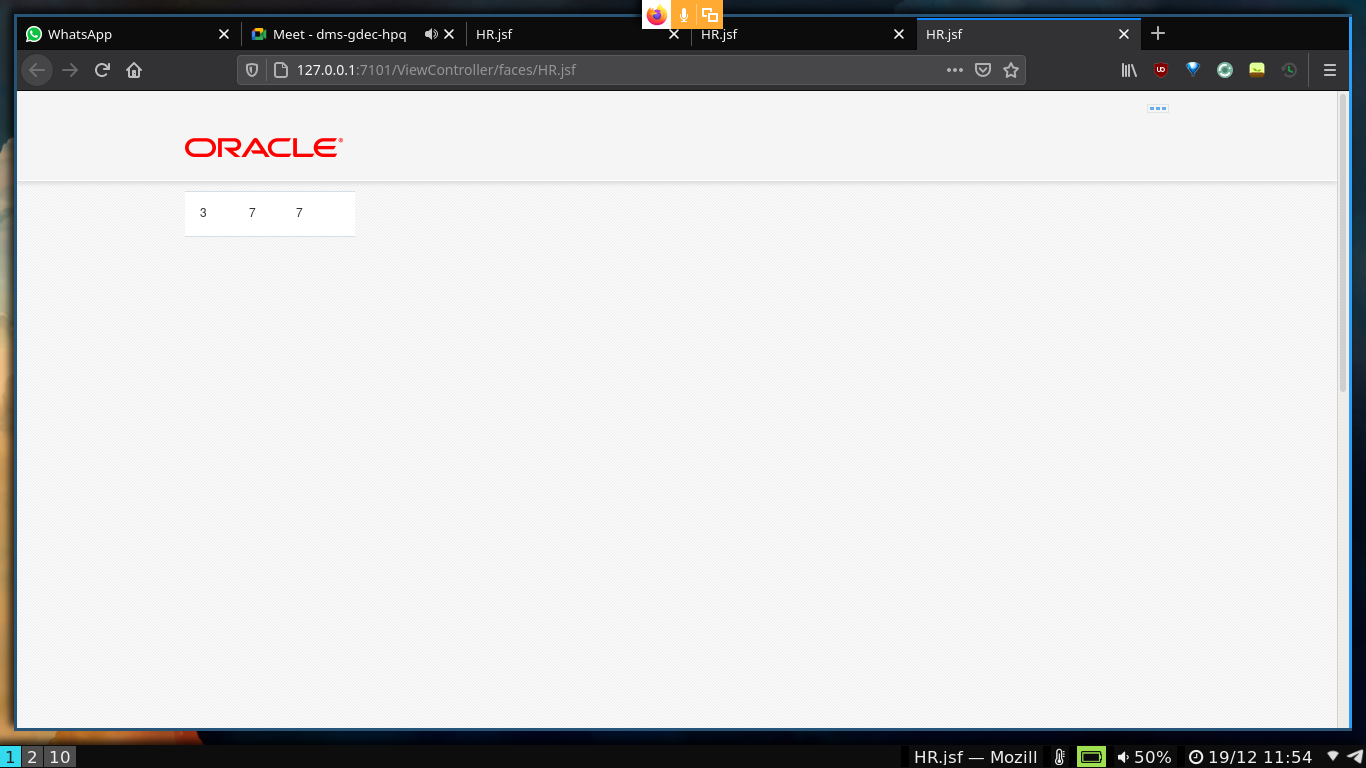
\includegraphics[scale=0.3]{33.png}
	\end{figure}
\end{enumerate}

\subsection{Modificar el diseño de la página}
En esta sección, vamos a modificar la página agregando algunos componentes para determinar el diseño de esta. Primero, agregamos un tablero para establecer el diseño general de la página. Luego agregamos los componentes que mostrarán datos sincronizados

\begin{enumerate}
	\item Volvemos a JDeveloper y en la ventana Estructura, seleccione la f:facet-center.
	\item Modificaremos el diseño del encabezado, para ello accedemos a \texttt{Components $\rightarrow$ Layout $\rightarrow$  Interactive Containers and Headers $\rightarrow$ Panel Dashboard}.

	Lo arrastramos y soltamos en f: facetCenter en la ventana Estructura
	\item A continuación \texttt{Components $\rightarrow$ Layout $\rightarrow$  Interactive Containers and Headers $\rightarrow$Panel box}. Lo arrastramos y soltamos en la ventana Estructura, en el componente af: panelDashboard que acabamos de agregar.
	\item Añadimos otros tres siendo así cuatro en total.
	\pagebreak
	\begin{figure}[!h]
	  \centering
	    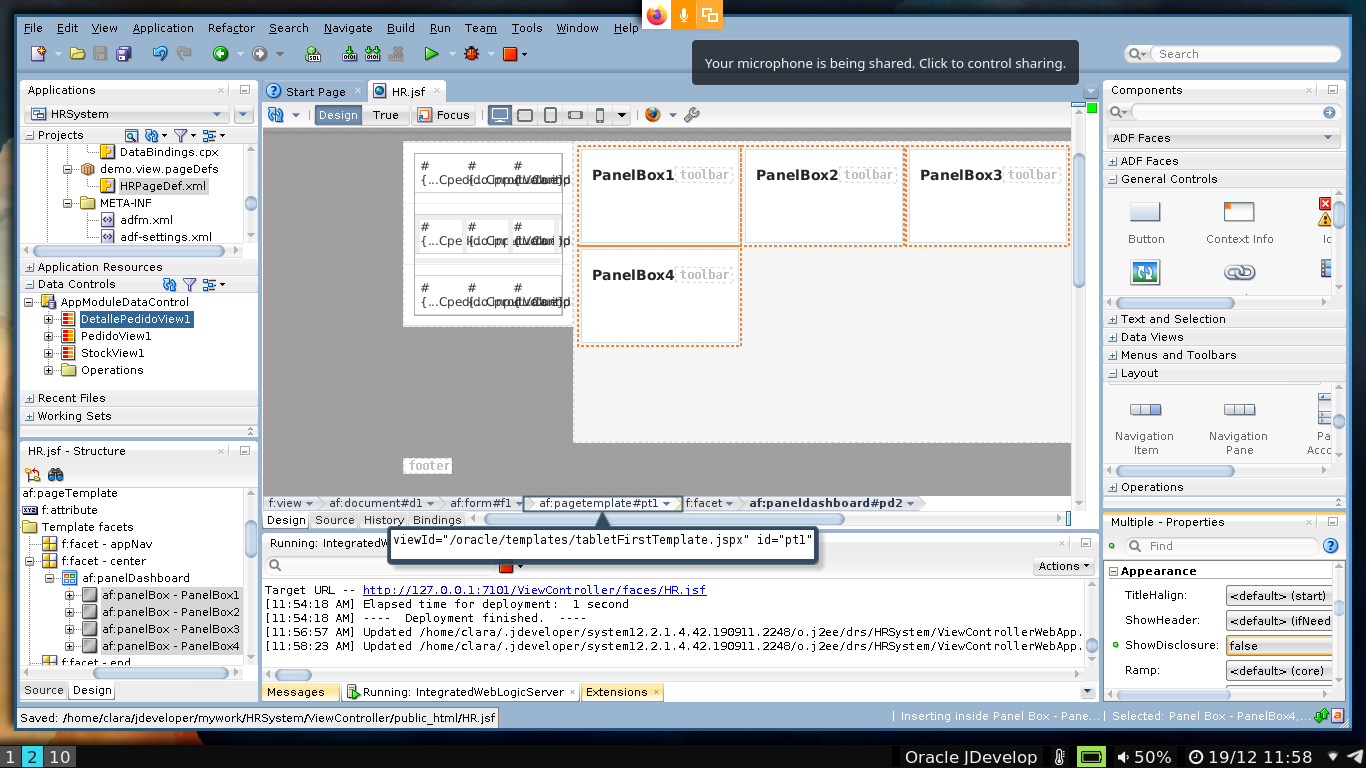
\includegraphics[scale=0.3]{34.png}
	\end{figure}
	\item Establecemos una propiedad para todas las cajas del panel. En la ventana Estructura, seleccionamos todos los af: panelBoxes. Luego, en la ventana ``Properties'', establecemos \texttt{Appearance $\rightarrow$ ShowDisclosure} a falso. Guardamos el trabajo
	\item De vuelta en la ventana Estructura, seleccionamos \texttt{af: panelDashboard} y establecemos las Columnas en 3 y RowHeight en 350px.  Guardamos el trabajo.
	\item Vamos al navegador y recargamos la página para ver los cuadros del panel. Como los cambios realizados son estéticos y no afectan a la base de datos, no hay necesidad de recompilar.
	\begin{figure}[!h]
	  \centering
	    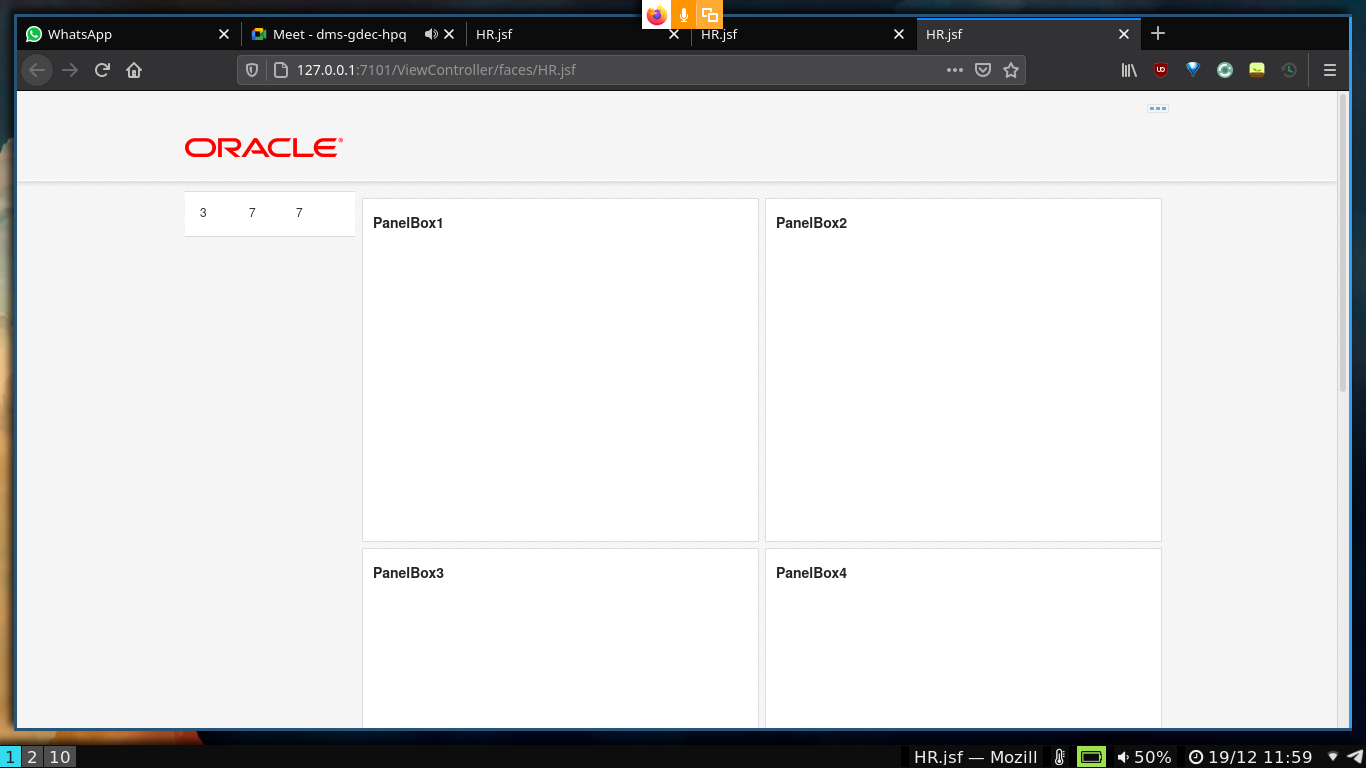
\includegraphics[scale=0.3]{35.png}
	\end{figure}
\end{enumerate}
\pagebreak

\subsection{Refinamiento del tablero y muestra de datos}
En esta parte del tutorial, mejoramos la interfaz de usuario agregando las tablas de la base de datos e incluyendo la funcionalidades de selección de columnas, reordenado de los campos en uno de los paneles y vinculado de los componentes comerciales a un gráfico.
Podemos hacer esto con simples operaciones de arrastrar y soltar: detrás de escena, la capa ADF Model maneja el enlace de datos por nosotros.

\begin{enumerate}
	\item Volvemos a la ventana Estructura de JDeveloper, seleccionamos af: panelBox - PanelBox1. Ponemos un título a la PanelBox1 mediante la propiedad ``Text''. Guardamos el trabajo.
	\item A continuación, agregamos algunos datos desde la ventana Controles de datos. En este caso vamos a mostrar la tabla Pedidos.

	Expandimos los nodos \texttt{AppModuleDataControl$\rightarrow$ PedidoView1} para exponer los datos que contiene.

	Arrastramos PedidoView1 a la ventana Estructura y lo soltamos en el nodo af: panelBox - pedido. En el menú emergente, seleccionamos \texttt{Vista de tabla / lista$\rightarrow$ Tabla ADF}.
	\item En el panel Create table, permitimos la selección de una sola fila. Habilitamos la clasificación, el filtrado y configuramos la tabla para que sea de solo lectura. Luego hacemos  clic en Aceptar.
	\begin{figure}[!h]
	  \centering
	    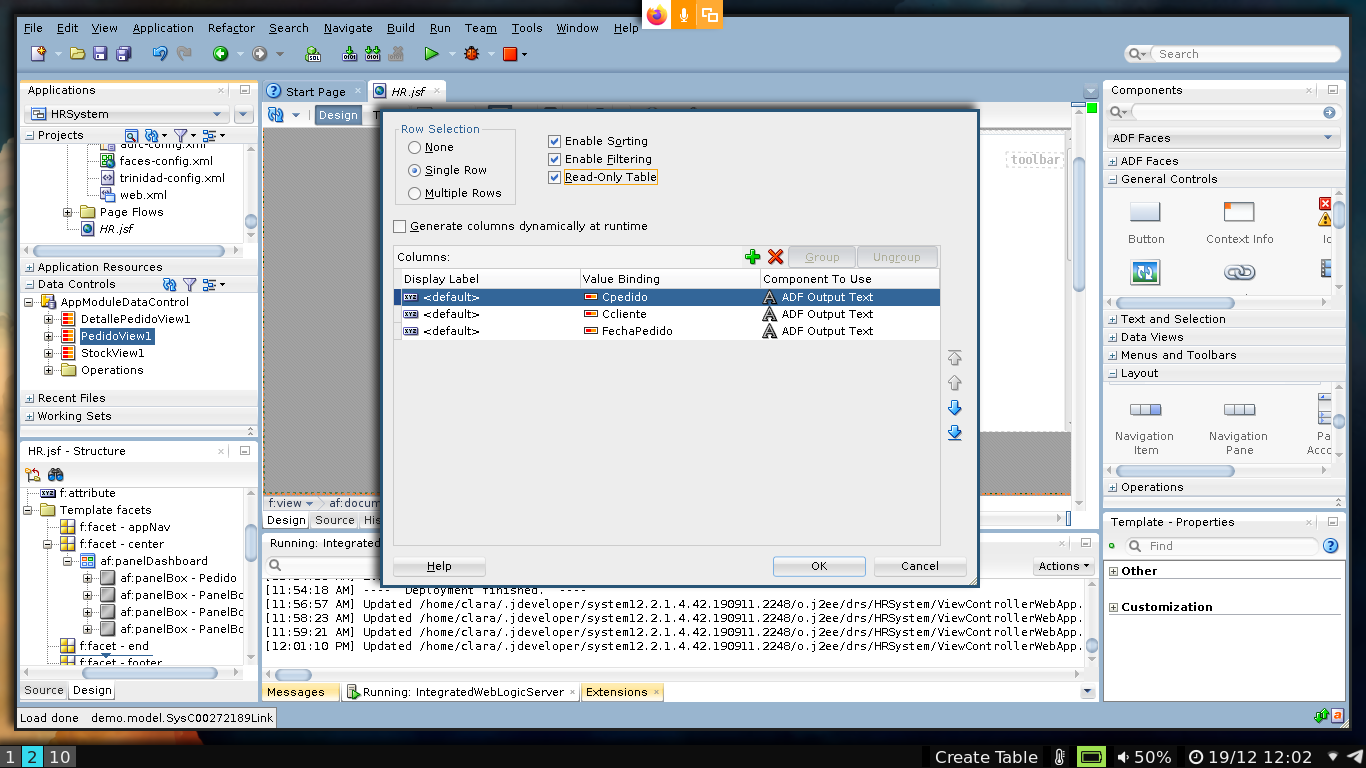
\includegraphics[scale=0.3]{36.png}
	\end{figure}
	\item Guardamos, y dado que se han agregado nuevos datos a la página, la debemos compilar nuevamente. Hacemos clic derecho en la página y seleccionamos \texttt{ejecutar/run}.

	Esto compilará nuestro proyecto, lo construirá e iniciará el servidor WebLogic integrado para ejecutarlo. Se abre el navegador web predeterminado para mostrar la página. Podemos seguir el progreso de estos pasos en la ventana Registro en JDeveloper.

	\item Ahora podemos ver los pedidos en el primer panel
	\pagebreak
	\begin{figure}[!h]
	  \centering
	    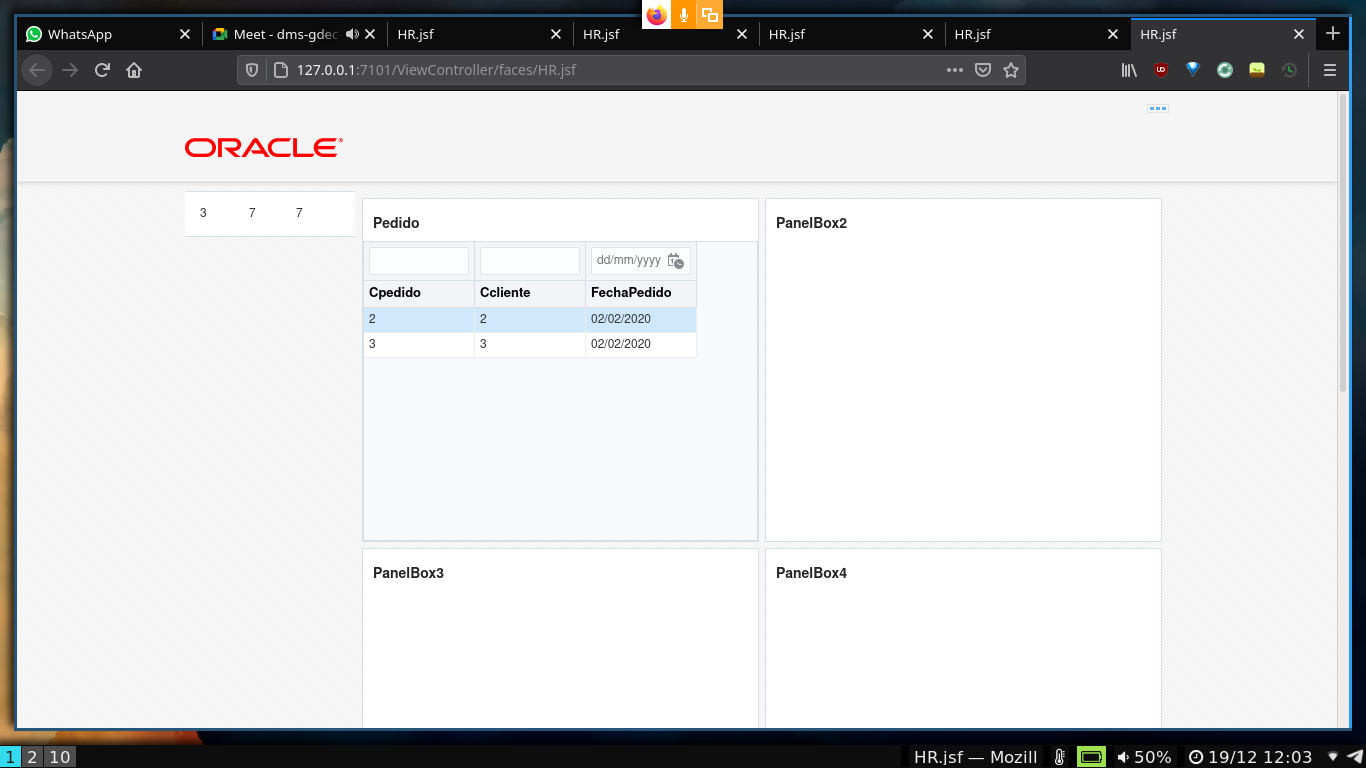
\includegraphics[scale=0.3]{37.png}
	\end{figure}

	Usamos las opciones que nos facilita para filtrar
	\begin{figure}[!h]
	  \centering
	    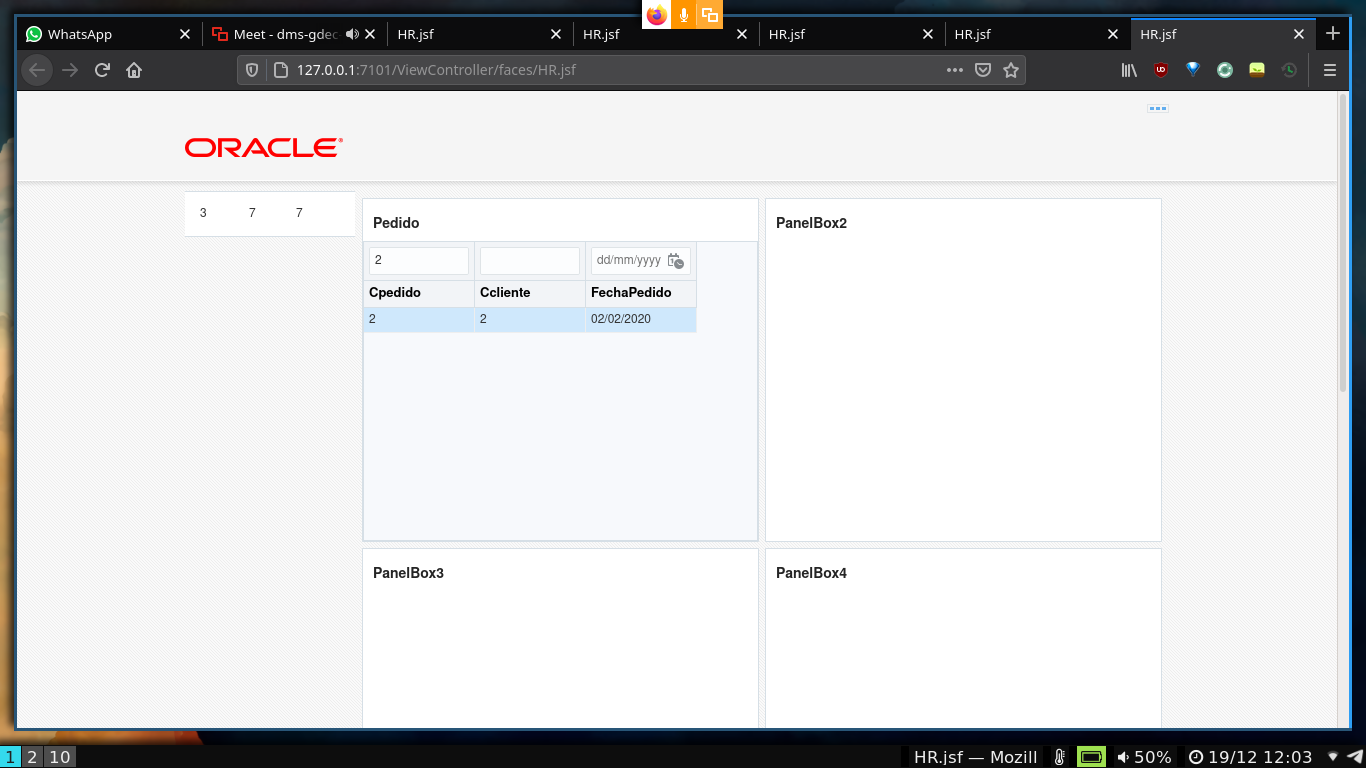
\includegraphics[scale=0.3]{38.png}
	\end{figure}
	\pagebreak
	\begin{figure}[!h]
	  \centering
	    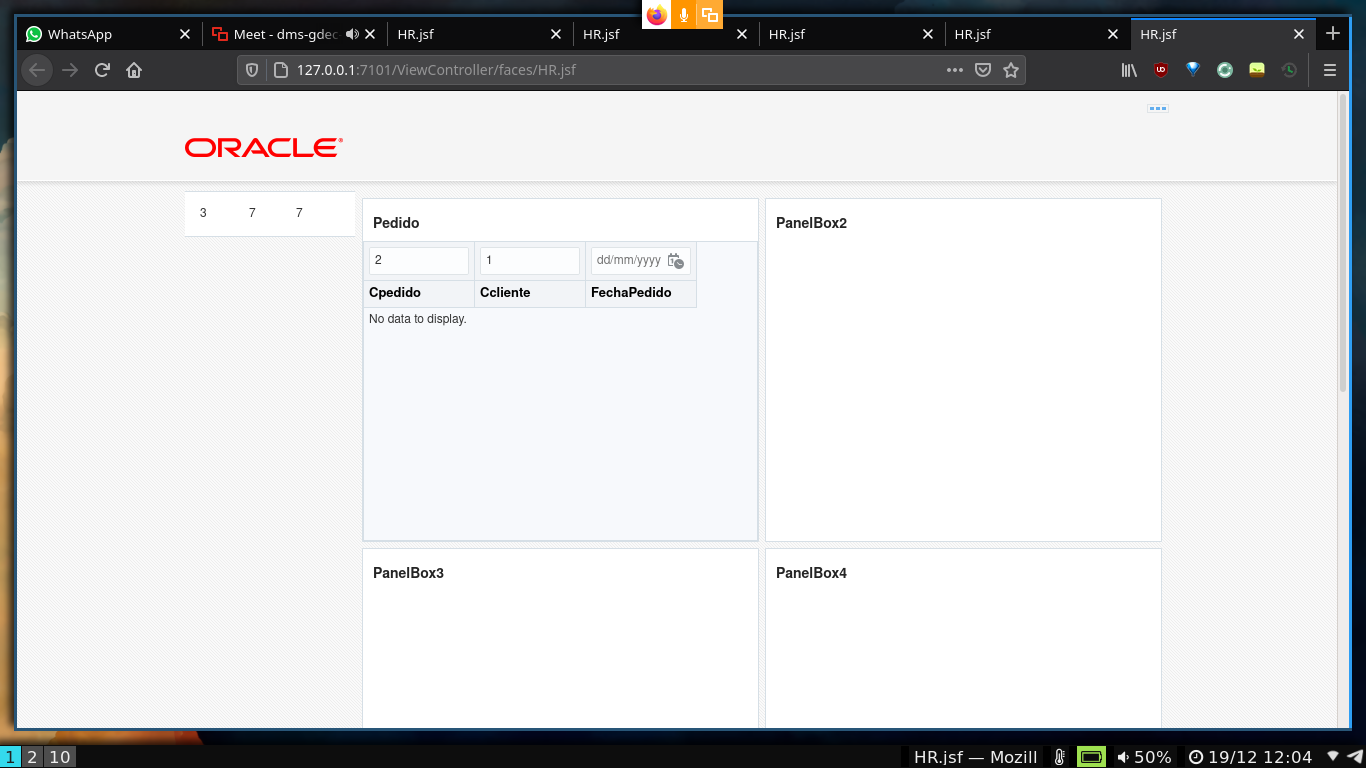
\includegraphics[scale=0.3]{39.png}
	\end{figure}
	\item Volvemos a Jdeveloper para trabajar con el segundo panelbox. Seleccionamos af: panelBox - PanelBox2. Establecemos un título, ``Stock'', con la propiedad Text. Guardamos.
	\item Arrastramos StockView1 a la ventana Estructura y lo soltamos en el nodo af: panelBox - stock. En el menú emergente, seleccionamos \texttt{Vista de tabla / lista$\rightarrow$ Tabla ADF}. En \texttt{Create Form pane}, le damos a OK y guardamos.
	\item Hacemos clic en el botón de Run, justo debajo de la barra de menú de JDeveloper, para efectuar estos cambios. Luego, volvemos a abrir la página en el navegador para ver que el segundo panel contiene datos detallados del stock.
	\begin{figure}[!h]
	  \centering
	    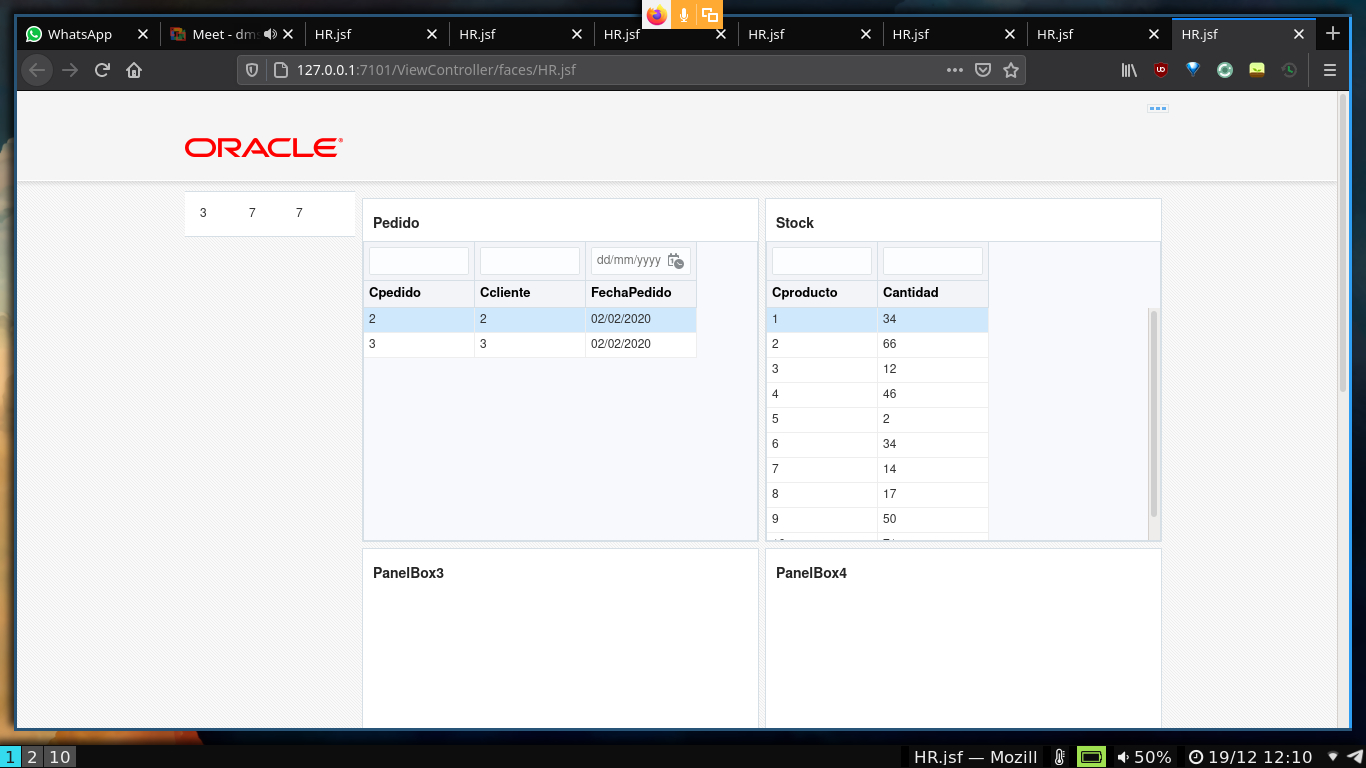
\includegraphics[scale=0.3]{40.png}
	\end{figure}
	\pagebreak
	\item Desde Controles de datos, arrastramos StockView1 a la ventana Estructura y lo soltamos en el cuadro del panel ``Stock2''. En el menú emergente, seleccione Chart.
	\item Al crear un gráfico, se puede usar el mismo control de datos para crear una variedad de gráficos diferentes. Nosotros hemos ido a \texttt{categories $\rightarrow$ Pie} y le damos OK
	\item Una vez decidido el gráfico, determinamos las sectores y los X axis que se utilizarán. En nuestro caso, en los sectores está la cantidad y en X axis ``Cproducto''.
	\begin{figure}[!h]
	  \centering
	    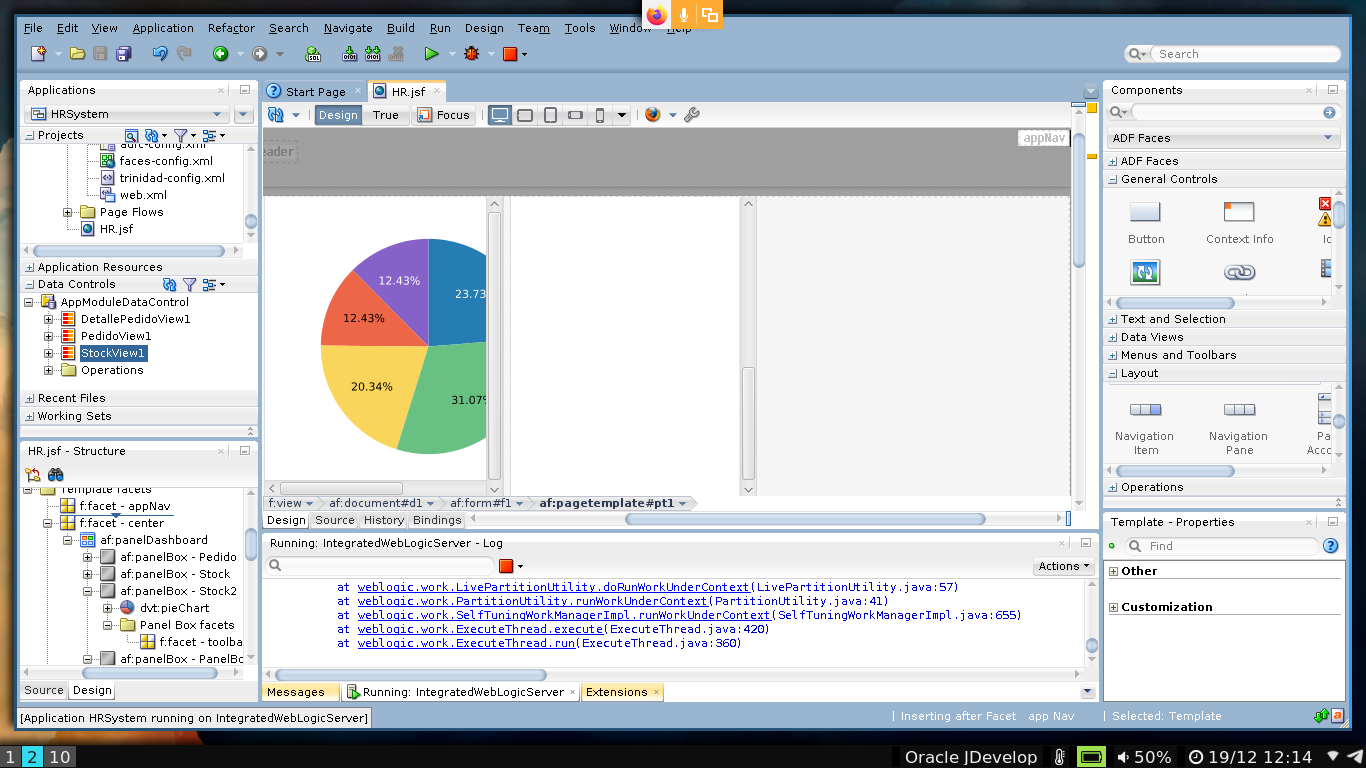
\includegraphics[scale=0.3]{41.png}
	\end{figure}
	\item Como hicimos anteriormente, guardamos, recompilamos y recargamos la web para ver los cambios.
\end{enumerate}

\subsection{Ajuste de los componentes del modelo para refinar como se muestran los datos}
\begin{enumerate}
	\item En la ventana \texttt{Applications $\rightarrow$ Model $\rightarrow$ Application Sources $\rightarrow$ demo.model}  hacemos doble click en Pedido y se nos abre en el editor Pedido.xml. Seleccionamos ``Attributes''.
	\item Seleccionamos \texttt{Ccliente $\rightarrow$ Validation} y seleccionamos el signo (+) verde para definir que tiene que estar entre 0 y 1000 (por ejemplo).
	\pagebreak
	\begin{figure}[!h]
	  \centering
	    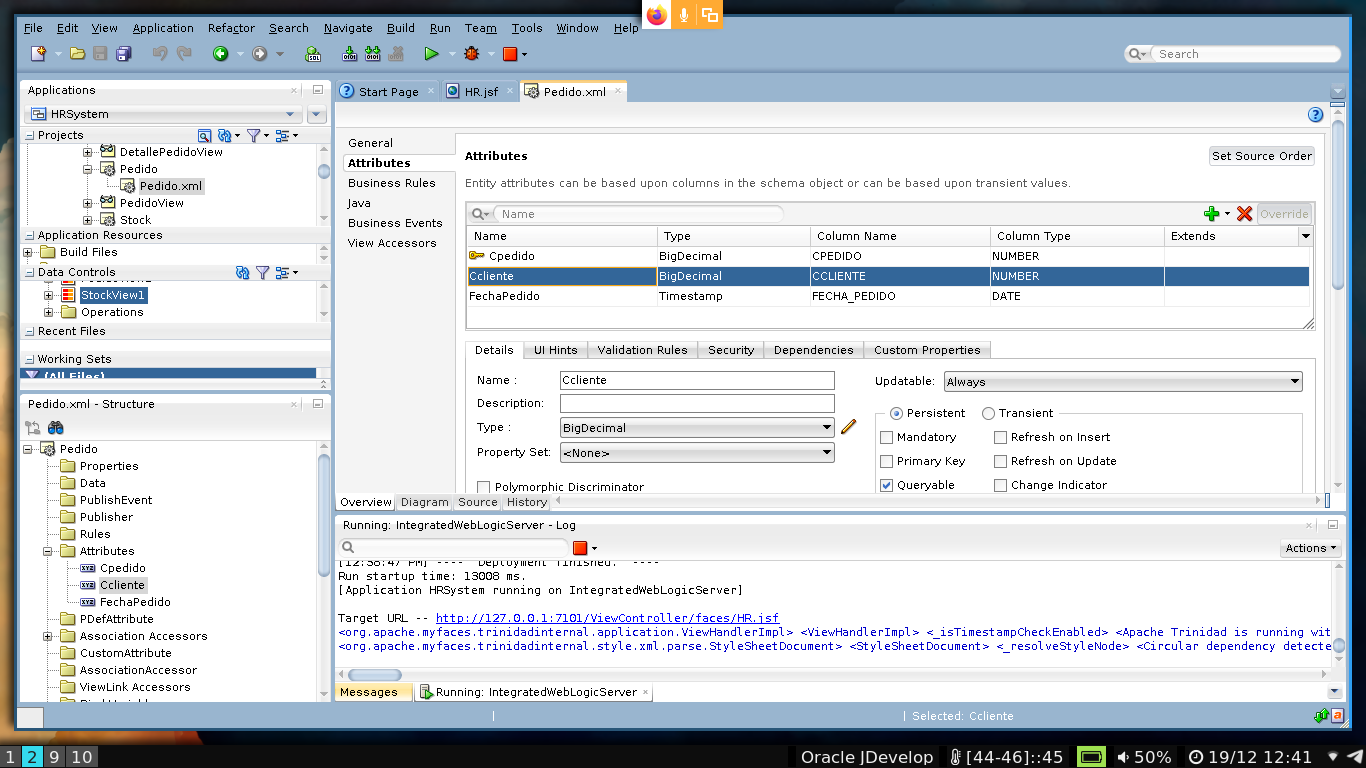
\includegraphics[scale=0.3]{42.png}
	\end{figure}
	\item Seleccionar Type: Range y Operator: Between $\rightarrow$ le ponemos los valores máximo y mínimo comentados.
	\begin{figure}[!h]
	  \centering
	    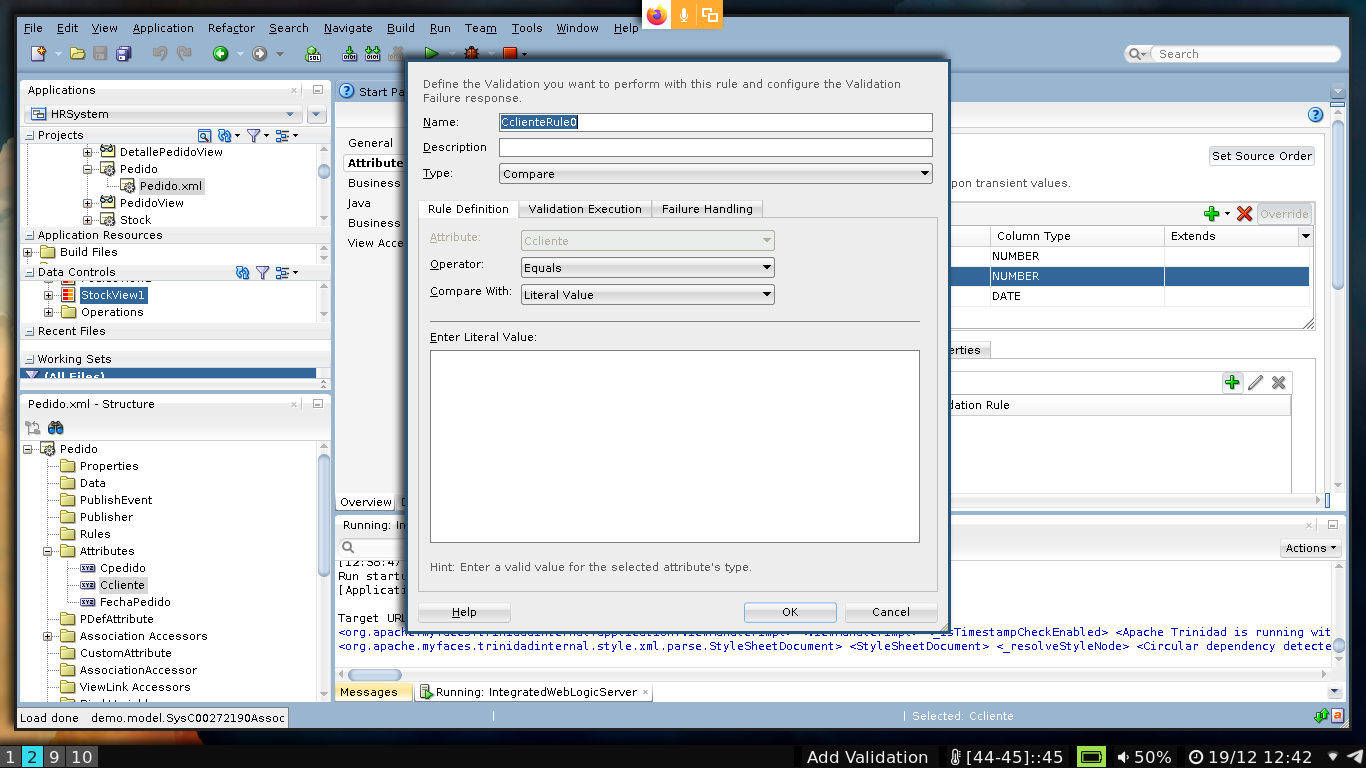
\includegraphics[scale=0.3]{43.png}
	\end{figure}
	\pagebreak
	\begin{figure}[!h]
	  \centering
	    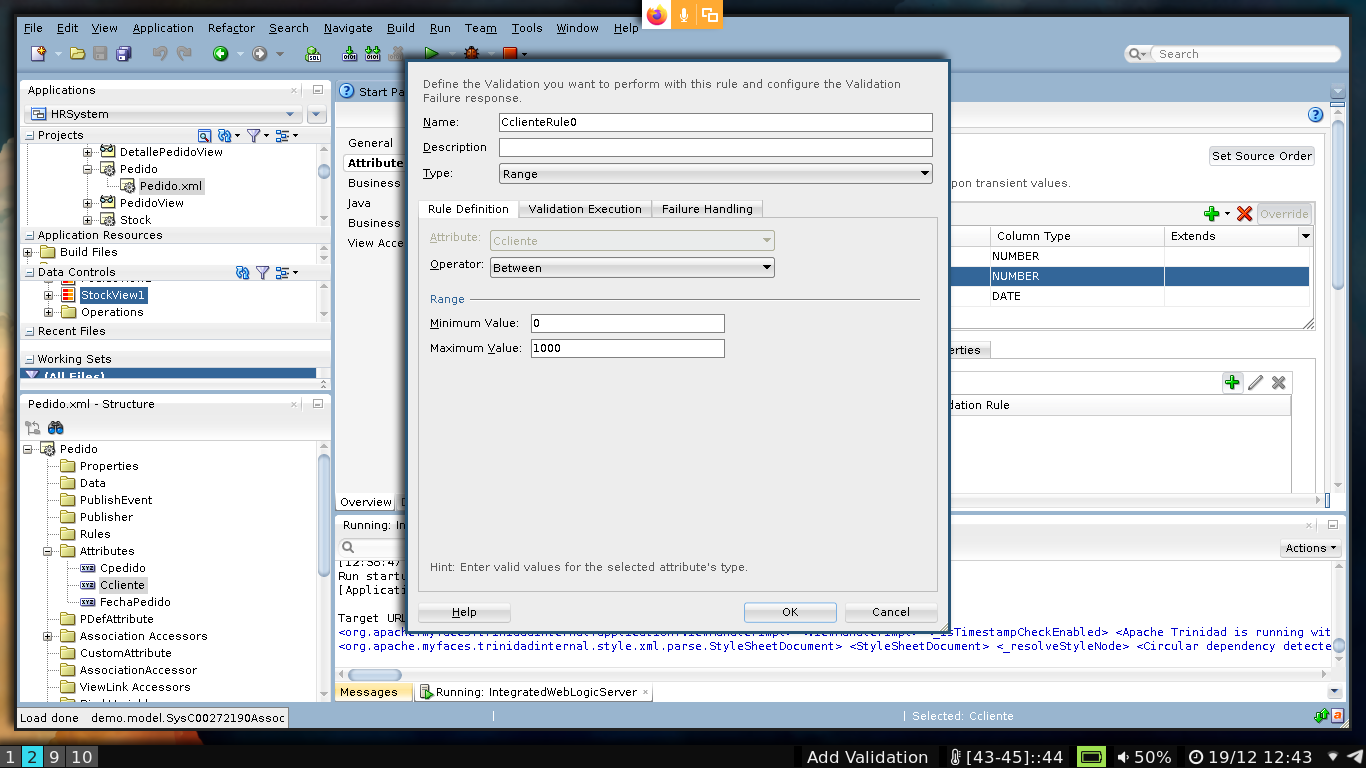
\includegraphics[scale=0.3]{44.png}
	\end{figure}
	\item Ponemos el mensaje de error en Failure Handling: ``Ya hay mil clientes, contacte con el administrador''
	\begin{figure}[!h]
	  \centering
	    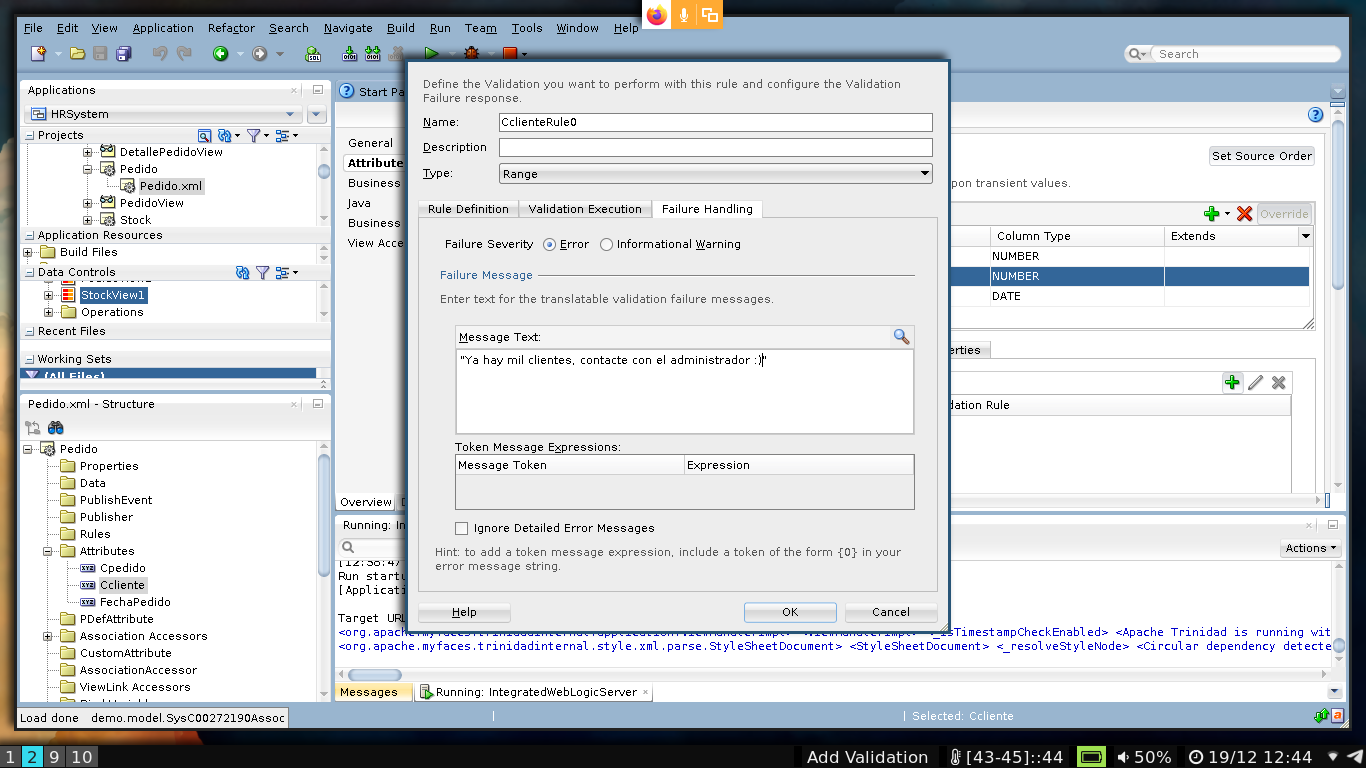
\includegraphics[scale=0.3]{44-5.png}
	\end{figure}
	\item Guardamos todo el trabajo.
	\item Definimos el formato de la fecha del pedido:
	\begin{enumerate}
		\item Label: Fecha
		\item Format Type: Simple Date
		\item Format: yyyy-mm-dd
	\end{enumerate}
	\begin{figure}[!h]
	  \centering
	    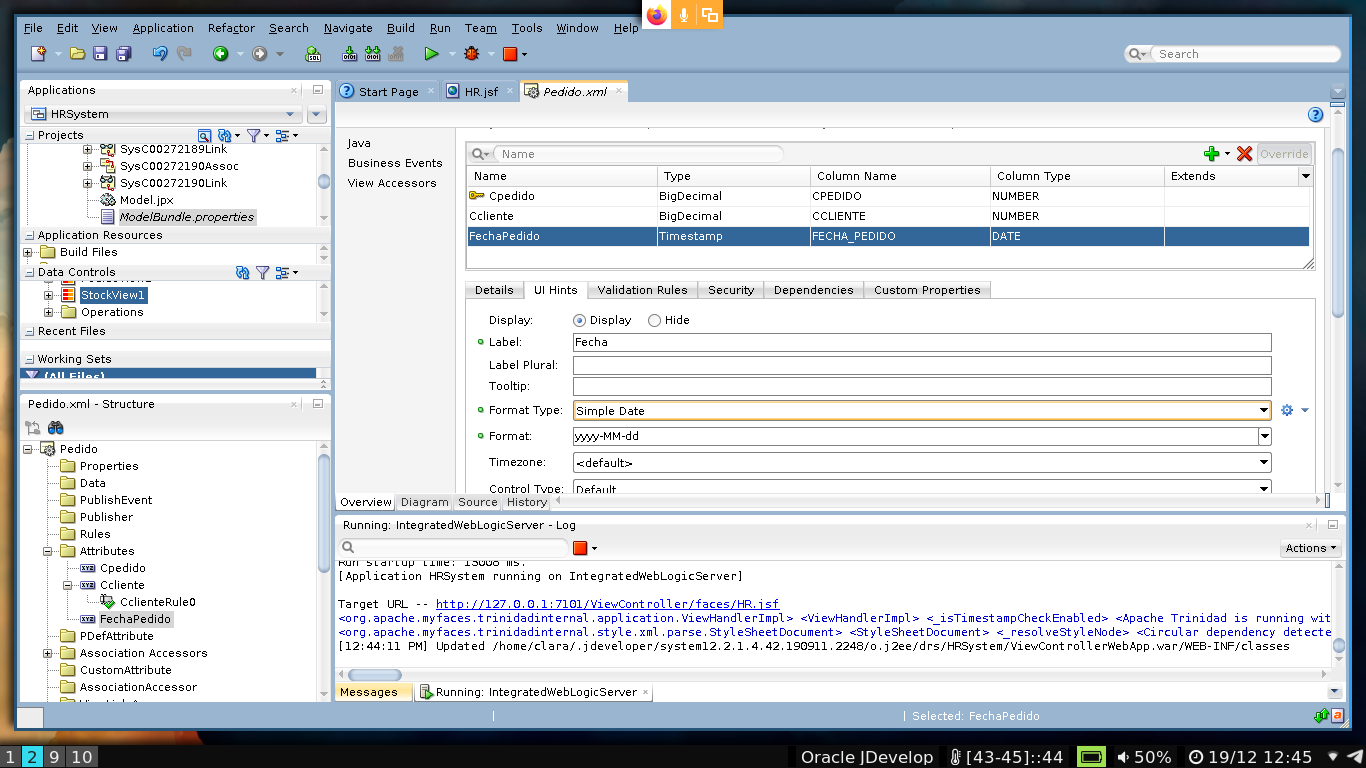
\includegraphics[scale=0.3]{45.png}
	\end{figure}
	\item Guardamos todo el trabajo de nuevo y cerramos la pestaña de Pedido.xml
\end{enumerate}
\pagebreak
\subsection{Retoques en la interfaz}
Finalmente, como hemos seguido el tutorial con un sistema distinto al que usaban (el sistema del Seminario 2), ciertas partes de la guía no encajaban bien con nuestra base de datos. Para compensar esto, añadimos todas nuestras tablas y ciertos ajustes de texto y estilo.
\begin{figure}[!h]
  \centering
	 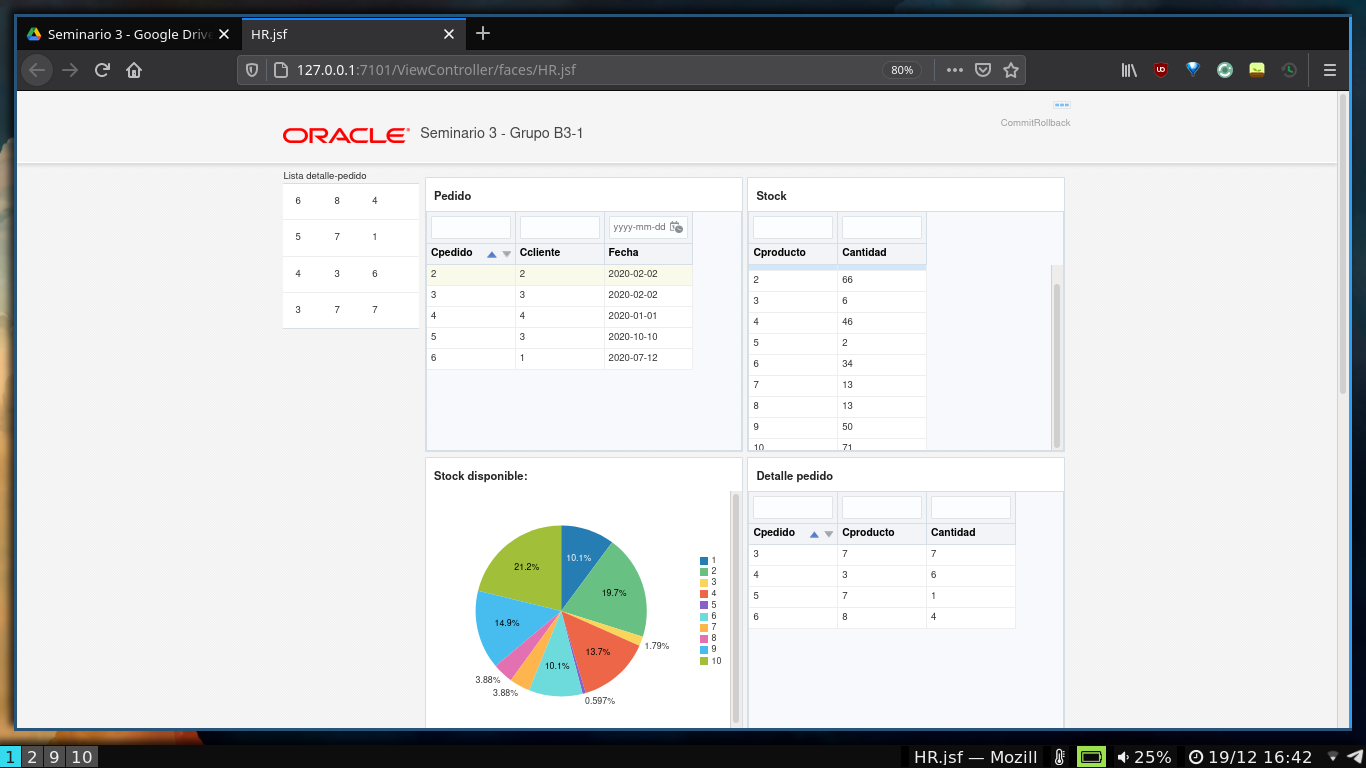
\includegraphics[scale=0.3]{46.png}
\end{figure}
